\documentclass[twoside]{book}

% Packages required by doxygen
\usepackage{calc}
\usepackage{doxygen}
\usepackage{graphicx}
\usepackage[utf8]{inputenc}
\usepackage{makeidx}
\usepackage{multicol}
\usepackage{multirow}
\usepackage{textcomp}
\usepackage[table]{xcolor}

% Font selection
\usepackage[T1]{fontenc}
\usepackage{mathptmx}
\usepackage[scaled=.90]{helvet}
\usepackage{courier}
\usepackage{amssymb}
\usepackage{sectsty}
\renewcommand{\familydefault}{\sfdefault}
\allsectionsfont{%
  \fontseries{bc}\selectfont%
  \color{darkgray}%
}
\renewcommand{\DoxyLabelFont}{%
  \fontseries{bc}\selectfont%
  \color{darkgray}%
}

% Page & text layout
\usepackage{geometry}
\geometry{%
  a4paper,%
  top=2.5cm,%
  bottom=2.5cm,%
  left=2.5cm,%
  right=2.5cm%
}
\tolerance=750
\hfuzz=15pt
\hbadness=750
\setlength{\emergencystretch}{15pt}
\setlength{\parindent}{0cm}
\setlength{\parskip}{0.2cm}
\makeatletter
\renewcommand{\paragraph}{%
  \@startsection{paragraph}{4}{0ex}{-1.0ex}{1.0ex}{%
    \normalfont\normalsize\bfseries\SS@parafont%
  }%
}
\renewcommand{\subparagraph}{%
  \@startsection{subparagraph}{5}{0ex}{-1.0ex}{1.0ex}{%
    \normalfont\normalsize\bfseries\SS@subparafont%
  }%
}
\makeatother

% Headers & footers
\usepackage{fancyhdr}
\pagestyle{fancyplain}
\fancyhead[LE]{\fancyplain{}{\bfseries\thepage}}
\fancyhead[CE]{\fancyplain{}{}}
\fancyhead[RE]{\fancyplain{}{\bfseries\leftmark}}
\fancyhead[LO]{\fancyplain{}{\bfseries\rightmark}}
\fancyhead[CO]{\fancyplain{}{}}
\fancyhead[RO]{\fancyplain{}{\bfseries\thepage}}
\fancyfoot[LE]{\fancyplain{}{}}
\fancyfoot[CE]{\fancyplain{}{}}
\fancyfoot[RE]{\fancyplain{}{\bfseries\scriptsize Generated on Thu Sep 19 2013 00\-:29\-:54 for Chess by Doxygen }}
\fancyfoot[LO]{\fancyplain{}{\bfseries\scriptsize Generated on Thu Sep 19 2013 00\-:29\-:54 for Chess by Doxygen }}
\fancyfoot[CO]{\fancyplain{}{}}
\fancyfoot[RO]{\fancyplain{}{}}
\renewcommand{\footrulewidth}{0.4pt}
\renewcommand{\chaptermark}[1]{%
  \markboth{#1}{}%
}
\renewcommand{\sectionmark}[1]{%
  \markright{\thesection\ #1}%
}

% Indices & bibliography
\usepackage{natbib}
\usepackage[titles]{tocloft}
\setcounter{tocdepth}{3}
\setcounter{secnumdepth}{5}
\makeindex

% Hyperlinks (required, but should be loaded last)
\usepackage{ifpdf}
\ifpdf
  \usepackage[pdftex,pagebackref=true]{hyperref}
\else
  \usepackage[ps2pdf,pagebackref=true]{hyperref}
\fi
\hypersetup{%
  colorlinks=true,%
  linkcolor=blue,%
  citecolor=blue,%
  unicode%
}

% Custom commands
\newcommand{\clearemptydoublepage}{%
  \newpage{\pagestyle{empty}\cleardoublepage}%
}


%===== C O N T E N T S =====

\begin{document}

% Titlepage & ToC
\hypersetup{pageanchor=false}
\pagenumbering{roman}
\begin{titlepage}
\vspace*{7cm}
\begin{center}%
{\Large Chess }\\
\vspace*{1cm}
{\large Generated by Doxygen 1.8.5}\\
\vspace*{0.5cm}
{\small Thu Sep 19 2013 00:29:54}\\
\end{center}
\end{titlepage}
\clearemptydoublepage
\tableofcontents
\clearemptydoublepage
\pagenumbering{arabic}
\hypersetup{pageanchor=true}

%--- Begin generated contents ---
\chapter{Documentation for Chess}
\label{index}\hypertarget{index}{}This chess game library contains a board, piece, mover and a View class that can be used to play a game of chess. 
\chapter{Namespace Index}
\section{Packages}
Here are the packages with brief descriptions (if available)\-:\begin{DoxyCompactList}
\item\contentsline{section}{\hyperlink{namespacegame}{game} }{\pageref{namespacegame}}{}
\item\contentsline{section}{\hyperlink{namespacepieces}{pieces} }{\pageref{namespacepieces}}{}
\end{DoxyCompactList}

\chapter{Hierarchical Index}
\section{Class Hierarchy}
This inheritance list is sorted roughly, but not completely, alphabetically\-:\begin{DoxyCompactList}
\item \contentsline{section}{game.\-Board}{\pageref{classgame_1_1_board}}{}
\item \contentsline{section}{game.\-Game}{\pageref{classgame_1_1_game}}{}
\item \contentsline{section}{pieces.\-Piece}{\pageref{classpieces_1_1_piece}}{}
\begin{DoxyCompactList}
\item \contentsline{section}{pieces.\-Bishop}{\pageref{classpieces_1_1_bishop}}{}
\item \contentsline{section}{pieces.\-Fly}{\pageref{classpieces_1_1_fly}}{}
\item \contentsline{section}{pieces.\-Fly\-Trap}{\pageref{classpieces_1_1_fly_trap}}{}
\item \contentsline{section}{pieces.\-King}{\pageref{classpieces_1_1_king}}{}
\item \contentsline{section}{pieces.\-Knight}{\pageref{classpieces_1_1_knight}}{}
\item \contentsline{section}{pieces.\-Pawn}{\pageref{classpieces_1_1_pawn}}{}
\item \contentsline{section}{pieces.\-Queen}{\pageref{classpieces_1_1_queen}}{}
\item \contentsline{section}{pieces.\-Rook}{\pageref{classpieces_1_1_rook}}{}
\end{DoxyCompactList}
\item \contentsline{section}{game.\-Player}{\pageref{classgame_1_1_player}}{}
\item \contentsline{section}{game.\-Position}{\pageref{classgame_1_1_position}}{}
\item \contentsline{section}{game.\-Game.\-State}{\pageref{classgame_1_1_game_1_1_state}}{}
\end{DoxyCompactList}

\chapter{Class Index}
\section{Class List}
Here are the classes, structs, unions and interfaces with brief descriptions\-:\begin{DoxyCompactList}
\item\contentsline{section}{\hyperlink{classpieces_1_1_bishop}{pieces.\-Bishop} }{\pageref{classpieces_1_1_bishop}}{}
\item\contentsline{section}{\hyperlink{classgame_1_1_board}{game.\-Board} }{\pageref{classgame_1_1_board}}{}
\item\contentsline{section}{\hyperlink{classpieces_1_1_fly}{pieces.\-Fly} }{\pageref{classpieces_1_1_fly}}{}
\item\contentsline{section}{\hyperlink{classpieces_1_1_fly_trap}{pieces.\-Fly\-Trap} }{\pageref{classpieces_1_1_fly_trap}}{}
\item\contentsline{section}{\hyperlink{classgame_1_1_game}{game.\-Game} }{\pageref{classgame_1_1_game}}{}
\item\contentsline{section}{\hyperlink{classpieces_1_1_king}{pieces.\-King} }{\pageref{classpieces_1_1_king}}{}
\item\contentsline{section}{\hyperlink{classpieces_1_1_knight}{pieces.\-Knight} }{\pageref{classpieces_1_1_knight}}{}
\item\contentsline{section}{\hyperlink{classpieces_1_1_pawn}{pieces.\-Pawn} }{\pageref{classpieces_1_1_pawn}}{}
\item\contentsline{section}{\hyperlink{classpieces_1_1_piece}{pieces.\-Piece} }{\pageref{classpieces_1_1_piece}}{}
\item\contentsline{section}{\hyperlink{classgame_1_1_player}{game.\-Player} }{\pageref{classgame_1_1_player}}{}
\item\contentsline{section}{\hyperlink{classgame_1_1_position}{game.\-Position} }{\pageref{classgame_1_1_position}}{}
\item\contentsline{section}{\hyperlink{classpieces_1_1_queen}{pieces.\-Queen} }{\pageref{classpieces_1_1_queen}}{}
\item\contentsline{section}{\hyperlink{classpieces_1_1_rook}{pieces.\-Rook} }{\pageref{classpieces_1_1_rook}}{}
\item\contentsline{section}{\hyperlink{classgame_1_1_game_1_1_state}{game.\-Game.\-State} }{\pageref{classgame_1_1_game_1_1_state}}{}
\end{DoxyCompactList}

\chapter{File Index}
\section{File List}
Here is a list of all files with brief descriptions\-:\begin{DoxyCompactList}
\item\contentsline{section}{/\-Volumes/\-Shared/\-Dropbox/\-Fall 13/\-C\-S 242/workspace/\-Chess/game/\hyperlink{_board_8java}{Board.\-java} }{\pageref{_board_8java}}{}
\item\contentsline{section}{/\-Volumes/\-Shared/\-Dropbox/\-Fall 13/\-C\-S 242/workspace/\-Chess/game/\hyperlink{_game_8java}{Game.\-java} }{\pageref{_game_8java}}{}
\item\contentsline{section}{/\-Volumes/\-Shared/\-Dropbox/\-Fall 13/\-C\-S 242/workspace/\-Chess/game/\hyperlink{_player_8java}{Player.\-java} }{\pageref{_player_8java}}{}
\item\contentsline{section}{/\-Volumes/\-Shared/\-Dropbox/\-Fall 13/\-C\-S 242/workspace/\-Chess/game/\hyperlink{_position_8java}{Position.\-java} }{\pageref{_position_8java}}{}
\item\contentsline{section}{/\-Volumes/\-Shared/\-Dropbox/\-Fall 13/\-C\-S 242/workspace/\-Chess/pieces/\hyperlink{_bishop_8java}{Bishop.\-java} }{\pageref{_bishop_8java}}{}
\item\contentsline{section}{/\-Volumes/\-Shared/\-Dropbox/\-Fall 13/\-C\-S 242/workspace/\-Chess/pieces/\hyperlink{_fly_8java}{Fly.\-java} }{\pageref{_fly_8java}}{}
\item\contentsline{section}{/\-Volumes/\-Shared/\-Dropbox/\-Fall 13/\-C\-S 242/workspace/\-Chess/pieces/\hyperlink{_fly_trap_8java}{Fly\-Trap.\-java} }{\pageref{_fly_trap_8java}}{}
\item\contentsline{section}{/\-Volumes/\-Shared/\-Dropbox/\-Fall 13/\-C\-S 242/workspace/\-Chess/pieces/\hyperlink{_king_8java}{King.\-java} }{\pageref{_king_8java}}{}
\item\contentsline{section}{/\-Volumes/\-Shared/\-Dropbox/\-Fall 13/\-C\-S 242/workspace/\-Chess/pieces/\hyperlink{_knight_8java}{Knight.\-java} }{\pageref{_knight_8java}}{}
\item\contentsline{section}{/\-Volumes/\-Shared/\-Dropbox/\-Fall 13/\-C\-S 242/workspace/\-Chess/pieces/\hyperlink{_pawn_8java}{Pawn.\-java} }{\pageref{_pawn_8java}}{}
\item\contentsline{section}{/\-Volumes/\-Shared/\-Dropbox/\-Fall 13/\-C\-S 242/workspace/\-Chess/pieces/\hyperlink{_piece_8java}{Piece.\-java} }{\pageref{_piece_8java}}{}
\item\contentsline{section}{/\-Volumes/\-Shared/\-Dropbox/\-Fall 13/\-C\-S 242/workspace/\-Chess/pieces/\hyperlink{_queen_8java}{Queen.\-java} }{\pageref{_queen_8java}}{}
\item\contentsline{section}{/\-Volumes/\-Shared/\-Dropbox/\-Fall 13/\-C\-S 242/workspace/\-Chess/pieces/\hyperlink{_rook_8java}{Rook.\-java} }{\pageref{_rook_8java}}{}
\end{DoxyCompactList}

\chapter{Namespace Documentation}
\hypertarget{namespacegame}{\section{Package game}
\label{namespacegame}\index{game@{game}}
}
\subsection*{Classes}
\begin{DoxyCompactItemize}
\item 
class \hyperlink{classgame_1_1_board}{Board}
\item 
class \hyperlink{classgame_1_1_game}{Game}
\item 
class \hyperlink{classgame_1_1_player}{Player}
\item 
class \hyperlink{classgame_1_1_position}{Position}
\item 
class {\bfseries Move}
\end{DoxyCompactItemize}

\hypertarget{namespacepieces}{\section{Package pieces}
\label{namespacepieces}\index{pieces@{pieces}}
}
\subsection*{Classes}
\begin{DoxyCompactItemize}
\item 
class \hyperlink{classpieces_1_1_bishop}{Bishop}
\item 
class \hyperlink{classpieces_1_1_fly}{Fly}
\item 
class \hyperlink{classpieces_1_1_fly_trap}{Fly\-Trap}
\item 
class \hyperlink{classpieces_1_1_king}{King}
\item 
class \hyperlink{classpieces_1_1_knight}{Knight}
\item 
class \hyperlink{classpieces_1_1_pawn}{Pawn}
\item 
class \hyperlink{classpieces_1_1_piece}{Piece}
\item 
class \hyperlink{classpieces_1_1_queen}{Queen}
\item 
class \hyperlink{classpieces_1_1_rook}{Rook}
\end{DoxyCompactItemize}

\chapter{Class Documentation}
\hypertarget{classpieces_1_1_bishop}{\section{pieces.\-Bishop Class Reference}
\label{classpieces_1_1_bishop}\index{pieces.\-Bishop@{pieces.\-Bishop}}
}
Inheritance diagram for pieces.\-Bishop\-:\begin{figure}[H]
\begin{center}
\leavevmode
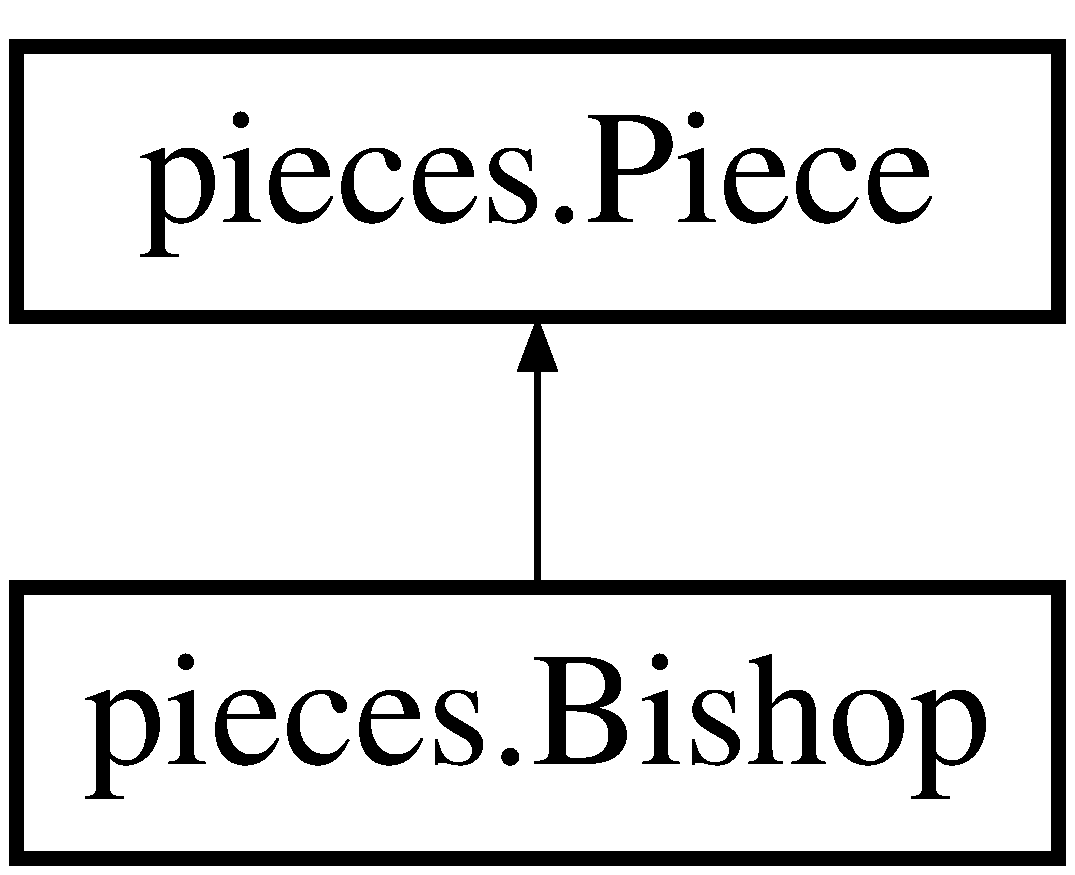
\includegraphics[height=2.000000cm]{classpieces_1_1_bishop}
\end{center}
\end{figure}
\subsection*{Public Member Functions}
\begin{DoxyCompactItemize}
\item 
\hyperlink{classpieces_1_1_bishop_ac46981a34fe380a8952fd19f6b96cd05}{Bishop} (int \hyperlink{classpieces_1_1_piece_ae40d6201d0aed36f369dd9d8f55892e3}{piece\-Type}, Board my\-Board, int x, int y)
\item 
\hyperlink{classpieces_1_1_bishop_ae5daf6af5a433314ec8bbe89d826a259}{Bishop} (int \hyperlink{classpieces_1_1_piece_ae40d6201d0aed36f369dd9d8f55892e3}{piece\-Type})
\item 
boolean \hyperlink{classpieces_1_1_bishop_a5222a9b4dc9cbe20a79234f7b3733124}{can\-Move\-Between} (Position start, Position end)
\end{DoxyCompactItemize}
\subsection*{Additional Inherited Members}


\subsection{Constructor \& Destructor Documentation}
\hypertarget{classpieces_1_1_bishop_ac46981a34fe380a8952fd19f6b96cd05}{\index{pieces\-::\-Bishop@{pieces\-::\-Bishop}!Bishop@{Bishop}}
\index{Bishop@{Bishop}!pieces::Bishop@{pieces\-::\-Bishop}}
\subsubsection[{Bishop}]{\setlength{\rightskip}{0pt plus 5cm}pieces.\-Bishop.\-Bishop (
\begin{DoxyParamCaption}
\item[{int}]{piece\-Type, }
\item[{Board}]{my\-Board, }
\item[{int}]{x, }
\item[{int}]{y}
\end{DoxyParamCaption}
)}}\label{classpieces_1_1_bishop_ac46981a34fe380a8952fd19f6b96cd05}
Constructor No check to verify if piece\-Type is a \hyperlink{classpieces_1_1_bishop}{Bishop}. It is up to the caller to verify. \hypertarget{classpieces_1_1_bishop_ae5daf6af5a433314ec8bbe89d826a259}{\index{pieces\-::\-Bishop@{pieces\-::\-Bishop}!Bishop@{Bishop}}
\index{Bishop@{Bishop}!pieces::Bishop@{pieces\-::\-Bishop}}
\subsubsection[{Bishop}]{\setlength{\rightskip}{0pt plus 5cm}pieces.\-Bishop.\-Bishop (
\begin{DoxyParamCaption}
\item[{int}]{piece\-Type}
\end{DoxyParamCaption}
)}}\label{classpieces_1_1_bishop_ae5daf6af5a433314ec8bbe89d826a259}
Constructor 

\subsection{Member Function Documentation}
\hypertarget{classpieces_1_1_bishop_a5222a9b4dc9cbe20a79234f7b3733124}{\index{pieces\-::\-Bishop@{pieces\-::\-Bishop}!can\-Move\-Between@{can\-Move\-Between}}
\index{can\-Move\-Between@{can\-Move\-Between}!pieces::Bishop@{pieces\-::\-Bishop}}
\subsubsection[{can\-Move\-Between}]{\setlength{\rightskip}{0pt plus 5cm}boolean pieces.\-Bishop.\-can\-Move\-Between (
\begin{DoxyParamCaption}
\item[{Position}]{start, }
\item[{Position}]{end}
\end{DoxyParamCaption}
)}}\label{classpieces_1_1_bishop_a5222a9b4dc9cbe20a79234f7b3733124}
Check if the piece can move from start to end location. \begin{DoxyReturn}{Returns}
true if it can. false otherwise. 
\end{DoxyReturn}


The documentation for this class was generated from the following file\-:\begin{DoxyCompactItemize}
\item 
/\-Volumes/\-Shared/\-Dropbox/\-Fall 13/\-C\-S 242/workspace/\-Chess/pieces/\hyperlink{_bishop_8java}{Bishop.\-java}\end{DoxyCompactItemize}

\hypertarget{classgame_1_1_board}{\section{game.\-Board Class Reference}
\label{classgame_1_1_board}\index{game.\-Board@{game.\-Board}}
}
\subsection*{Public Member Functions}
\begin{DoxyCompactItemize}
\item 
\hyperlink{classgame_1_1_board_a03ab3e485bfe19fc57cc4985b252633b}{Board} (int board\-Type)
\item 
boolean \hyperlink{classgame_1_1_board_ad42721c60eee469c46075ee976c4fe37}{empty\-At} (\hyperlink{classgame_1_1_position}{Position} pos)
\item 
boolean \hyperlink{classgame_1_1_board_a9a0acc7212f18f11d2ea71248ee0641b}{occupied\-At} (\hyperlink{classgame_1_1_position}{Position} pos)
\item 
int \hyperlink{classgame_1_1_board_ae945b5be4a7c7ded9abf70486f564389}{get\-Piece\-Type\-At} (\hyperlink{classgame_1_1_position}{Position} pos)
\item 
\hyperlink{classpieces_1_1_piece}{Piece} \hyperlink{classgame_1_1_board_ab33022a9aed668318676e718d7d67b20}{get\-Piece\-At} (\hyperlink{classgame_1_1_position}{Position} pos)
\item 
boolean \hyperlink{classgame_1_1_board_ac84d149dded8dc8b106cec222d20933c}{points\-Are\-Opponents} (\hyperlink{classgame_1_1_position}{Position} a, \hyperlink{classgame_1_1_position}{Position} b)
\item 
boolean \hyperlink{classgame_1_1_board_ae8c779458e916755cd15c672dbe7628b}{points\-Are\-Allies} (\hyperlink{classgame_1_1_position}{Position} a, \hyperlink{classgame_1_1_position}{Position} b)
\item 
boolean \hyperlink{classgame_1_1_board_a707fca7d3091d8af2ba7e66fcea90e31}{straight\-Or\-Diag\-Is\-Clear} (\hyperlink{classgame_1_1_position}{Position} start, \hyperlink{classgame_1_1_position}{Position} end)
\item 
\hyperlink{classpieces_1_1_piece}{Piece} \hyperlink{classgame_1_1_board_aeb0730b986f552300a5a68d7a68bd8d7}{remove\-Piece\-From} (\hyperlink{classgame_1_1_position}{Position} pos)
\item 
void \hyperlink{classgame_1_1_board_a88e794ba7dec65d4b8582016615dec0f}{add\-Piece\-To} (\hyperlink{classgame_1_1_position}{Position} pos, \hyperlink{classpieces_1_1_piece}{Piece} p)
\item 
void \hyperlink{classgame_1_1_board_a33d619089bcaef94b641ecd6d014cfac}{print\-Board} ()
\end{DoxyCompactItemize}
\subsection*{Static Public Member Functions}
\begin{DoxyCompactItemize}
\item 
static int \hyperlink{classgame_1_1_board_ad08736b75fde9ed768c7842759b442f8}{get\-Size} ()
\end{DoxyCompactItemize}
\subsection*{Public Attributes}
\begin{DoxyCompactItemize}
\item 
\hyperlink{classpieces_1_1_piece}{Piece} \hyperlink{classgame_1_1_board_ae468c82687902428871a19693c923c15}{white\-King}
\item 
\hyperlink{classpieces_1_1_piece}{Piece} \hyperlink{classgame_1_1_board_a3208a9b2a809f279c2f33f2f87a9a68c}{black\-King}
\item 
\hyperlink{classpieces_1_1_piece}{Piece}\mbox{[}$\,$\mbox{]}\mbox{[}$\,$\mbox{]} \hyperlink{classgame_1_1_board_a7b235a9a7c1dbfd5373366fe8bd2c4e2}{board}
\item 
int\mbox{[}$\,$\mbox{]}\mbox{[}$\,$\mbox{]} \hyperlink{classgame_1_1_board_aef78af0593e283d51122b0aff9e98d3e}{board\-Int\-Array}
\item 
int \hyperlink{classgame_1_1_board_acd643578da78ae9b61cbc0b962d03bc7}{check} = \hyperlink{classpieces_1_1_piece_a5d79a14b2b47d6699449dd3e015f0392}{Piece.\-E\-M\-P\-T\-Y}
\end{DoxyCompactItemize}
\subsection*{Static Public Attributes}
\begin{DoxyCompactItemize}
\item 
static final int \hyperlink{classgame_1_1_board_ad8df367d654710a005091c644088879e}{C\-L\-A\-S\-S\-I\-C} = 1
\item 
static final int \hyperlink{classgame_1_1_board_a1bac85e381255ac84399072df7b863e9}{C\-U\-S\-T\-O\-M} = 2
\item 
static final int \hyperlink{classgame_1_1_board_a1919fd52c264639c24155b333495a11c}{E\-M\-P\-T\-Y} = 0
\item 
static final int \hyperlink{classgame_1_1_board_abeabe8126dcd677e8570991415155513}{P\-A\-W\-N} = 1
\item 
static final int \hyperlink{classgame_1_1_board_a6e93b6ff58a5e29c8067eaf569acd7d1}{R\-O\-O\-K} = 2
\item 
static final int \hyperlink{classgame_1_1_board_a805c2fa05787d3a91d4cbf34d74970f3}{K\-N\-I\-G\-H\-T} = 3
\item 
static final int \hyperlink{classgame_1_1_board_a43354b0544e528583e783c228b3016a3}{B\-I\-S\-H\-O\-P} = 4
\item 
static final int \hyperlink{classgame_1_1_board_a010790144c6c1e42d97ce588d1522184}{Q\-U\-E\-E\-N} = 5
\item 
static final int \hyperlink{classgame_1_1_board_aa90eb06edcc6b4159963daa2bb83fa37}{K\-I\-N\-G} = 6
\item 
static final int \hyperlink{classgame_1_1_board_aa68c679fcb4744729d246aba79e7613a}{F\-L\-Y} = 7
\item 
static final int \hyperlink{classgame_1_1_board_a7f0beeebc30980894df8aec277501cd5}{F\-L\-Y\-T\-R\-A\-P} = 8
\item 
static final int \hyperlink{classgame_1_1_board_ad3b4223ca4e14051a8bdd78a95b38071}{W\-H\-I\-T\-E} = 1
\item 
static final int \hyperlink{classgame_1_1_board_a6495a2020e20b656f5e82cf55cae41f0}{B\-L\-A\-C\-K} = -\/1
\end{DoxyCompactItemize}
\subsection*{Private Member Functions}
\begin{DoxyCompactItemize}
\item 
void \hyperlink{classgame_1_1_board_afdb8d18115d6485c6c428345ee14172b}{fill\-Board} (int board\-Type)
\end{DoxyCompactItemize}


\subsection{Detailed Description}
The \hyperlink{classgame_1_1_board}{Board} class represents the Chess board and tracks the pieces. \begin{DoxyAuthor}{Author}
Shashank Bharadwaj 
\end{DoxyAuthor}
\begin{DoxyDate}{Date}
Wed, 4 Sep 2013 
\end{DoxyDate}


\subsection{Constructor \& Destructor Documentation}
\hypertarget{classgame_1_1_board_a03ab3e485bfe19fc57cc4985b252633b}{\index{game\-::\-Board@{game\-::\-Board}!Board@{Board}}
\index{Board@{Board}!game::Board@{game\-::\-Board}}
\subsubsection[{Board}]{\setlength{\rightskip}{0pt plus 5cm}game.\-Board.\-Board (
\begin{DoxyParamCaption}
\item[{int}]{board\-Type}
\end{DoxyParamCaption}
)}}\label{classgame_1_1_board_a03ab3e485bfe19fc57cc4985b252633b}
Constructor creates an 8x8 array with chess pieces in initial configuration. Piece numbering\-: 1-\/6. White pieces are + and Black are -\/ Eg. Black rook will be -\/2 

\subsection{Member Function Documentation}
\hypertarget{classgame_1_1_board_a88e794ba7dec65d4b8582016615dec0f}{\index{game\-::\-Board@{game\-::\-Board}!add\-Piece\-To@{add\-Piece\-To}}
\index{add\-Piece\-To@{add\-Piece\-To}!game::Board@{game\-::\-Board}}
\subsubsection[{add\-Piece\-To}]{\setlength{\rightskip}{0pt plus 5cm}void game.\-Board.\-add\-Piece\-To (
\begin{DoxyParamCaption}
\item[{{\bf Position}}]{pos, }
\item[{{\bf Piece}}]{p}
\end{DoxyParamCaption}
)}}\label{classgame_1_1_board_a88e794ba7dec65d4b8582016615dec0f}
adds a piece to its data structures. Must be called from a move function 
\begin{DoxyParams}{Parameters}
{\em pos,\-:} & position to add piece \\
\hline
\end{DoxyParams}
\hypertarget{classgame_1_1_board_ad42721c60eee469c46075ee976c4fe37}{\index{game\-::\-Board@{game\-::\-Board}!empty\-At@{empty\-At}}
\index{empty\-At@{empty\-At}!game::Board@{game\-::\-Board}}
\subsubsection[{empty\-At}]{\setlength{\rightskip}{0pt plus 5cm}boolean game.\-Board.\-empty\-At (
\begin{DoxyParamCaption}
\item[{{\bf Position}}]{pos}
\end{DoxyParamCaption}
)}}\label{classgame_1_1_board_ad42721c60eee469c46075ee976c4fe37}
Checks if a position is empty 
\begin{DoxyParams}{Parameters}
{\em pos,\-:} & position on the board \\
\hline
\end{DoxyParams}
\begin{DoxyReturn}{Returns}
true if empty, false otherwise 
\end{DoxyReturn}
\hypertarget{classgame_1_1_board_afdb8d18115d6485c6c428345ee14172b}{\index{game\-::\-Board@{game\-::\-Board}!fill\-Board@{fill\-Board}}
\index{fill\-Board@{fill\-Board}!game::Board@{game\-::\-Board}}
\subsubsection[{fill\-Board}]{\setlength{\rightskip}{0pt plus 5cm}void game.\-Board.\-fill\-Board (
\begin{DoxyParamCaption}
\item[{int}]{board\-Type}
\end{DoxyParamCaption}
)\hspace{0.3cm}{\ttfamily [private]}}}\label{classgame_1_1_board_afdb8d18115d6485c6c428345ee14172b}
Fills the board with pieces 
\begin{DoxyParams}{Parameters}
{\em board\-Type,\-:} & Classic board or Custom board \\
\hline
\end{DoxyParams}
\hypertarget{classgame_1_1_board_ab33022a9aed668318676e718d7d67b20}{\index{game\-::\-Board@{game\-::\-Board}!get\-Piece\-At@{get\-Piece\-At}}
\index{get\-Piece\-At@{get\-Piece\-At}!game::Board@{game\-::\-Board}}
\subsubsection[{get\-Piece\-At}]{\setlength{\rightskip}{0pt plus 5cm}{\bf Piece} game.\-Board.\-get\-Piece\-At (
\begin{DoxyParamCaption}
\item[{{\bf Position}}]{pos}
\end{DoxyParamCaption}
)}}\label{classgame_1_1_board_ab33022a9aed668318676e718d7d67b20}
Gets the piece object at a position on the board \begin{DoxyReturn}{Returns}
Piece object on success, null if empty 
\end{DoxyReturn}
\hypertarget{classgame_1_1_board_ae945b5be4a7c7ded9abf70486f564389}{\index{game\-::\-Board@{game\-::\-Board}!get\-Piece\-Type\-At@{get\-Piece\-Type\-At}}
\index{get\-Piece\-Type\-At@{get\-Piece\-Type\-At}!game::Board@{game\-::\-Board}}
\subsubsection[{get\-Piece\-Type\-At}]{\setlength{\rightskip}{0pt plus 5cm}int game.\-Board.\-get\-Piece\-Type\-At (
\begin{DoxyParamCaption}
\item[{{\bf Position}}]{pos}
\end{DoxyParamCaption}
)}}\label{classgame_1_1_board_ae945b5be4a7c7ded9abf70486f564389}
Gets the piece\-Type at a position on the board \begin{DoxyReturn}{Returns}
piece\-Type on success, 0 if empty 
\end{DoxyReturn}
\hypertarget{classgame_1_1_board_ad08736b75fde9ed768c7842759b442f8}{\index{game\-::\-Board@{game\-::\-Board}!get\-Size@{get\-Size}}
\index{get\-Size@{get\-Size}!game::Board@{game\-::\-Board}}
\subsubsection[{get\-Size}]{\setlength{\rightskip}{0pt plus 5cm}static int game.\-Board.\-get\-Size (
\begin{DoxyParamCaption}
{}
\end{DoxyParamCaption}
)\hspace{0.3cm}{\ttfamily [static]}}}\label{classgame_1_1_board_ad08736b75fde9ed768c7842759b442f8}
Getter \hypertarget{classgame_1_1_board_a9a0acc7212f18f11d2ea71248ee0641b}{\index{game\-::\-Board@{game\-::\-Board}!occupied\-At@{occupied\-At}}
\index{occupied\-At@{occupied\-At}!game::Board@{game\-::\-Board}}
\subsubsection[{occupied\-At}]{\setlength{\rightskip}{0pt plus 5cm}boolean game.\-Board.\-occupied\-At (
\begin{DoxyParamCaption}
\item[{{\bf Position}}]{pos}
\end{DoxyParamCaption}
)}}\label{classgame_1_1_board_a9a0acc7212f18f11d2ea71248ee0641b}
Checks if a position is occupied 
\begin{DoxyParams}{Parameters}
{\em pos,\-:} & position on the board \\
\hline
\end{DoxyParams}
\begin{DoxyReturn}{Returns}
true if occupied, false otherwise 
\end{DoxyReturn}
\hypertarget{classgame_1_1_board_ae8c779458e916755cd15c672dbe7628b}{\index{game\-::\-Board@{game\-::\-Board}!points\-Are\-Allies@{points\-Are\-Allies}}
\index{points\-Are\-Allies@{points\-Are\-Allies}!game::Board@{game\-::\-Board}}
\subsubsection[{points\-Are\-Allies}]{\setlength{\rightskip}{0pt plus 5cm}boolean game.\-Board.\-points\-Are\-Allies (
\begin{DoxyParamCaption}
\item[{{\bf Position}}]{a, }
\item[{{\bf Position}}]{b}
\end{DoxyParamCaption}
)}}\label{classgame_1_1_board_ae8c779458e916755cd15c672dbe7628b}
Checks if Piece p and piece at pos are allies. Spaces must be occupied \begin{DoxyReturn}{Returns}
true if they are allies, false otherwise 
\end{DoxyReturn}
\hypertarget{classgame_1_1_board_ac84d149dded8dc8b106cec222d20933c}{\index{game\-::\-Board@{game\-::\-Board}!points\-Are\-Opponents@{points\-Are\-Opponents}}
\index{points\-Are\-Opponents@{points\-Are\-Opponents}!game::Board@{game\-::\-Board}}
\subsubsection[{points\-Are\-Opponents}]{\setlength{\rightskip}{0pt plus 5cm}boolean game.\-Board.\-points\-Are\-Opponents (
\begin{DoxyParamCaption}
\item[{{\bf Position}}]{a, }
\item[{{\bf Position}}]{b}
\end{DoxyParamCaption}
)}}\label{classgame_1_1_board_ac84d149dded8dc8b106cec222d20933c}
Checks if Piece p and piece at pos are opponents. Spaces must be occupied \begin{DoxyReturn}{Returns}
true if they are opponents, false otherwise 
\end{DoxyReturn}
\hypertarget{classgame_1_1_board_a33d619089bcaef94b641ecd6d014cfac}{\index{game\-::\-Board@{game\-::\-Board}!print\-Board@{print\-Board}}
\index{print\-Board@{print\-Board}!game::Board@{game\-::\-Board}}
\subsubsection[{print\-Board}]{\setlength{\rightskip}{0pt plus 5cm}void game.\-Board.\-print\-Board (
\begin{DoxyParamCaption}
{}
\end{DoxyParamCaption}
)}}\label{classgame_1_1_board_a33d619089bcaef94b641ecd6d014cfac}
Prints the 8x8 chessboard. Black pieces on the top row, white on the bottom \hypertarget{classgame_1_1_board_aeb0730b986f552300a5a68d7a68bd8d7}{\index{game\-::\-Board@{game\-::\-Board}!remove\-Piece\-From@{remove\-Piece\-From}}
\index{remove\-Piece\-From@{remove\-Piece\-From}!game::Board@{game\-::\-Board}}
\subsubsection[{remove\-Piece\-From}]{\setlength{\rightskip}{0pt plus 5cm}{\bf Piece} game.\-Board.\-remove\-Piece\-From (
\begin{DoxyParamCaption}
\item[{{\bf Position}}]{pos}
\end{DoxyParamCaption}
)}}\label{classgame_1_1_board_aeb0730b986f552300a5a68d7a68bd8d7}
Removes a piece from its data structures. Must be called from a move function 
\begin{DoxyParams}{Parameters}
{\em pos,\-:} & position from which to remove piece \\
\hline
\end{DoxyParams}
\hypertarget{classgame_1_1_board_a707fca7d3091d8af2ba7e66fcea90e31}{\index{game\-::\-Board@{game\-::\-Board}!straight\-Or\-Diag\-Is\-Clear@{straight\-Or\-Diag\-Is\-Clear}}
\index{straight\-Or\-Diag\-Is\-Clear@{straight\-Or\-Diag\-Is\-Clear}!game::Board@{game\-::\-Board}}
\subsubsection[{straight\-Or\-Diag\-Is\-Clear}]{\setlength{\rightskip}{0pt plus 5cm}boolean game.\-Board.\-straight\-Or\-Diag\-Is\-Clear (
\begin{DoxyParamCaption}
\item[{{\bf Position}}]{start, }
\item[{{\bf Position}}]{end}
\end{DoxyParamCaption}
)}}\label{classgame_1_1_board_a707fca7d3091d8af2ba7e66fcea90e31}
Checks if a straight or diagonal path is clear. Must not be a one step move. 
\begin{DoxyParams}{Parameters}
{\em start} & and end positions, and the board \\
\hline
\end{DoxyParams}
\begin{DoxyReturn}{Returns}
true if path is clear, false otherwise. 
\end{DoxyReturn}


\subsection{Member Data Documentation}
\hypertarget{classgame_1_1_board_a43354b0544e528583e783c228b3016a3}{\index{game\-::\-Board@{game\-::\-Board}!B\-I\-S\-H\-O\-P@{B\-I\-S\-H\-O\-P}}
\index{B\-I\-S\-H\-O\-P@{B\-I\-S\-H\-O\-P}!game::Board@{game\-::\-Board}}
\subsubsection[{B\-I\-S\-H\-O\-P}]{\setlength{\rightskip}{0pt plus 5cm}final int game.\-Board.\-B\-I\-S\-H\-O\-P = 4\hspace{0.3cm}{\ttfamily [static]}}}\label{classgame_1_1_board_a43354b0544e528583e783c228b3016a3}
\hypertarget{classgame_1_1_board_a6495a2020e20b656f5e82cf55cae41f0}{\index{game\-::\-Board@{game\-::\-Board}!B\-L\-A\-C\-K@{B\-L\-A\-C\-K}}
\index{B\-L\-A\-C\-K@{B\-L\-A\-C\-K}!game::Board@{game\-::\-Board}}
\subsubsection[{B\-L\-A\-C\-K}]{\setlength{\rightskip}{0pt plus 5cm}final int game.\-Board.\-B\-L\-A\-C\-K = -\/1\hspace{0.3cm}{\ttfamily [static]}}}\label{classgame_1_1_board_a6495a2020e20b656f5e82cf55cae41f0}
\hypertarget{classgame_1_1_board_a3208a9b2a809f279c2f33f2f87a9a68c}{\index{game\-::\-Board@{game\-::\-Board}!black\-King@{black\-King}}
\index{black\-King@{black\-King}!game::Board@{game\-::\-Board}}
\subsubsection[{black\-King}]{\setlength{\rightskip}{0pt plus 5cm}{\bf Piece} game.\-Board.\-black\-King}}\label{classgame_1_1_board_a3208a9b2a809f279c2f33f2f87a9a68c}
\hypertarget{classgame_1_1_board_a7b235a9a7c1dbfd5373366fe8bd2c4e2}{\index{game\-::\-Board@{game\-::\-Board}!board@{board}}
\index{board@{board}!game::Board@{game\-::\-Board}}
\subsubsection[{board}]{\setlength{\rightskip}{0pt plus 5cm}{\bf Piece} \mbox{[}$\,$\mbox{]}\mbox{[}$\,$\mbox{]} game.\-Board.\-board}}\label{classgame_1_1_board_a7b235a9a7c1dbfd5373366fe8bd2c4e2}
\hypertarget{classgame_1_1_board_aef78af0593e283d51122b0aff9e98d3e}{\index{game\-::\-Board@{game\-::\-Board}!board\-Int\-Array@{board\-Int\-Array}}
\index{board\-Int\-Array@{board\-Int\-Array}!game::Board@{game\-::\-Board}}
\subsubsection[{board\-Int\-Array}]{\setlength{\rightskip}{0pt plus 5cm}int \mbox{[}$\,$\mbox{]}\mbox{[}$\,$\mbox{]} game.\-Board.\-board\-Int\-Array}}\label{classgame_1_1_board_aef78af0593e283d51122b0aff9e98d3e}
\hypertarget{classgame_1_1_board_acd643578da78ae9b61cbc0b962d03bc7}{\index{game\-::\-Board@{game\-::\-Board}!check@{check}}
\index{check@{check}!game::Board@{game\-::\-Board}}
\subsubsection[{check}]{\setlength{\rightskip}{0pt plus 5cm}int game.\-Board.\-check = {\bf Piece.\-E\-M\-P\-T\-Y}}}\label{classgame_1_1_board_acd643578da78ae9b61cbc0b962d03bc7}
\hypertarget{classgame_1_1_board_ad8df367d654710a005091c644088879e}{\index{game\-::\-Board@{game\-::\-Board}!C\-L\-A\-S\-S\-I\-C@{C\-L\-A\-S\-S\-I\-C}}
\index{C\-L\-A\-S\-S\-I\-C@{C\-L\-A\-S\-S\-I\-C}!game::Board@{game\-::\-Board}}
\subsubsection[{C\-L\-A\-S\-S\-I\-C}]{\setlength{\rightskip}{0pt plus 5cm}final int game.\-Board.\-C\-L\-A\-S\-S\-I\-C = 1\hspace{0.3cm}{\ttfamily [static]}}}\label{classgame_1_1_board_ad8df367d654710a005091c644088879e}
\hypertarget{classgame_1_1_board_a1bac85e381255ac84399072df7b863e9}{\index{game\-::\-Board@{game\-::\-Board}!C\-U\-S\-T\-O\-M@{C\-U\-S\-T\-O\-M}}
\index{C\-U\-S\-T\-O\-M@{C\-U\-S\-T\-O\-M}!game::Board@{game\-::\-Board}}
\subsubsection[{C\-U\-S\-T\-O\-M}]{\setlength{\rightskip}{0pt plus 5cm}final int game.\-Board.\-C\-U\-S\-T\-O\-M = 2\hspace{0.3cm}{\ttfamily [static]}}}\label{classgame_1_1_board_a1bac85e381255ac84399072df7b863e9}
\hypertarget{classgame_1_1_board_a1919fd52c264639c24155b333495a11c}{\index{game\-::\-Board@{game\-::\-Board}!E\-M\-P\-T\-Y@{E\-M\-P\-T\-Y}}
\index{E\-M\-P\-T\-Y@{E\-M\-P\-T\-Y}!game::Board@{game\-::\-Board}}
\subsubsection[{E\-M\-P\-T\-Y}]{\setlength{\rightskip}{0pt plus 5cm}final int game.\-Board.\-E\-M\-P\-T\-Y = 0\hspace{0.3cm}{\ttfamily [static]}}}\label{classgame_1_1_board_a1919fd52c264639c24155b333495a11c}
\hypertarget{classgame_1_1_board_aa68c679fcb4744729d246aba79e7613a}{\index{game\-::\-Board@{game\-::\-Board}!F\-L\-Y@{F\-L\-Y}}
\index{F\-L\-Y@{F\-L\-Y}!game::Board@{game\-::\-Board}}
\subsubsection[{F\-L\-Y}]{\setlength{\rightskip}{0pt plus 5cm}final int game.\-Board.\-F\-L\-Y = 7\hspace{0.3cm}{\ttfamily [static]}}}\label{classgame_1_1_board_aa68c679fcb4744729d246aba79e7613a}
\hypertarget{classgame_1_1_board_a7f0beeebc30980894df8aec277501cd5}{\index{game\-::\-Board@{game\-::\-Board}!F\-L\-Y\-T\-R\-A\-P@{F\-L\-Y\-T\-R\-A\-P}}
\index{F\-L\-Y\-T\-R\-A\-P@{F\-L\-Y\-T\-R\-A\-P}!game::Board@{game\-::\-Board}}
\subsubsection[{F\-L\-Y\-T\-R\-A\-P}]{\setlength{\rightskip}{0pt plus 5cm}final int game.\-Board.\-F\-L\-Y\-T\-R\-A\-P = 8\hspace{0.3cm}{\ttfamily [static]}}}\label{classgame_1_1_board_a7f0beeebc30980894df8aec277501cd5}
\hypertarget{classgame_1_1_board_aa90eb06edcc6b4159963daa2bb83fa37}{\index{game\-::\-Board@{game\-::\-Board}!K\-I\-N\-G@{K\-I\-N\-G}}
\index{K\-I\-N\-G@{K\-I\-N\-G}!game::Board@{game\-::\-Board}}
\subsubsection[{K\-I\-N\-G}]{\setlength{\rightskip}{0pt plus 5cm}final int game.\-Board.\-K\-I\-N\-G = 6\hspace{0.3cm}{\ttfamily [static]}}}\label{classgame_1_1_board_aa90eb06edcc6b4159963daa2bb83fa37}
\hypertarget{classgame_1_1_board_a805c2fa05787d3a91d4cbf34d74970f3}{\index{game\-::\-Board@{game\-::\-Board}!K\-N\-I\-G\-H\-T@{K\-N\-I\-G\-H\-T}}
\index{K\-N\-I\-G\-H\-T@{K\-N\-I\-G\-H\-T}!game::Board@{game\-::\-Board}}
\subsubsection[{K\-N\-I\-G\-H\-T}]{\setlength{\rightskip}{0pt plus 5cm}final int game.\-Board.\-K\-N\-I\-G\-H\-T = 3\hspace{0.3cm}{\ttfamily [static]}}}\label{classgame_1_1_board_a805c2fa05787d3a91d4cbf34d74970f3}
\hypertarget{classgame_1_1_board_abeabe8126dcd677e8570991415155513}{\index{game\-::\-Board@{game\-::\-Board}!P\-A\-W\-N@{P\-A\-W\-N}}
\index{P\-A\-W\-N@{P\-A\-W\-N}!game::Board@{game\-::\-Board}}
\subsubsection[{P\-A\-W\-N}]{\setlength{\rightskip}{0pt plus 5cm}final int game.\-Board.\-P\-A\-W\-N = 1\hspace{0.3cm}{\ttfamily [static]}}}\label{classgame_1_1_board_abeabe8126dcd677e8570991415155513}
\hypertarget{classgame_1_1_board_a010790144c6c1e42d97ce588d1522184}{\index{game\-::\-Board@{game\-::\-Board}!Q\-U\-E\-E\-N@{Q\-U\-E\-E\-N}}
\index{Q\-U\-E\-E\-N@{Q\-U\-E\-E\-N}!game::Board@{game\-::\-Board}}
\subsubsection[{Q\-U\-E\-E\-N}]{\setlength{\rightskip}{0pt plus 5cm}final int game.\-Board.\-Q\-U\-E\-E\-N = 5\hspace{0.3cm}{\ttfamily [static]}}}\label{classgame_1_1_board_a010790144c6c1e42d97ce588d1522184}
\hypertarget{classgame_1_1_board_a6e93b6ff58a5e29c8067eaf569acd7d1}{\index{game\-::\-Board@{game\-::\-Board}!R\-O\-O\-K@{R\-O\-O\-K}}
\index{R\-O\-O\-K@{R\-O\-O\-K}!game::Board@{game\-::\-Board}}
\subsubsection[{R\-O\-O\-K}]{\setlength{\rightskip}{0pt plus 5cm}final int game.\-Board.\-R\-O\-O\-K = 2\hspace{0.3cm}{\ttfamily [static]}}}\label{classgame_1_1_board_a6e93b6ff58a5e29c8067eaf569acd7d1}
\hypertarget{classgame_1_1_board_ad3b4223ca4e14051a8bdd78a95b38071}{\index{game\-::\-Board@{game\-::\-Board}!W\-H\-I\-T\-E@{W\-H\-I\-T\-E}}
\index{W\-H\-I\-T\-E@{W\-H\-I\-T\-E}!game::Board@{game\-::\-Board}}
\subsubsection[{W\-H\-I\-T\-E}]{\setlength{\rightskip}{0pt plus 5cm}final int game.\-Board.\-W\-H\-I\-T\-E = 1\hspace{0.3cm}{\ttfamily [static]}}}\label{classgame_1_1_board_ad3b4223ca4e14051a8bdd78a95b38071}
\hypertarget{classgame_1_1_board_ae468c82687902428871a19693c923c15}{\index{game\-::\-Board@{game\-::\-Board}!white\-King@{white\-King}}
\index{white\-King@{white\-King}!game::Board@{game\-::\-Board}}
\subsubsection[{white\-King}]{\setlength{\rightskip}{0pt plus 5cm}{\bf Piece} game.\-Board.\-white\-King}}\label{classgame_1_1_board_ae468c82687902428871a19693c923c15}


The documentation for this class was generated from the following file\-:\begin{DoxyCompactItemize}
\item 
/\-Volumes/\-Shared/\-Dropbox/\-Fall 13/\-C\-S 242/workspace/\-Chess/game/\hyperlink{_board_8java}{Board.\-java}\end{DoxyCompactItemize}

\hypertarget{classpieces_1_1_fly}{\section{pieces.\-Fly Class Reference}
\label{classpieces_1_1_fly}\index{pieces.\-Fly@{pieces.\-Fly}}
}
Inheritance diagram for pieces.\-Fly\-:\begin{figure}[H]
\begin{center}
\leavevmode
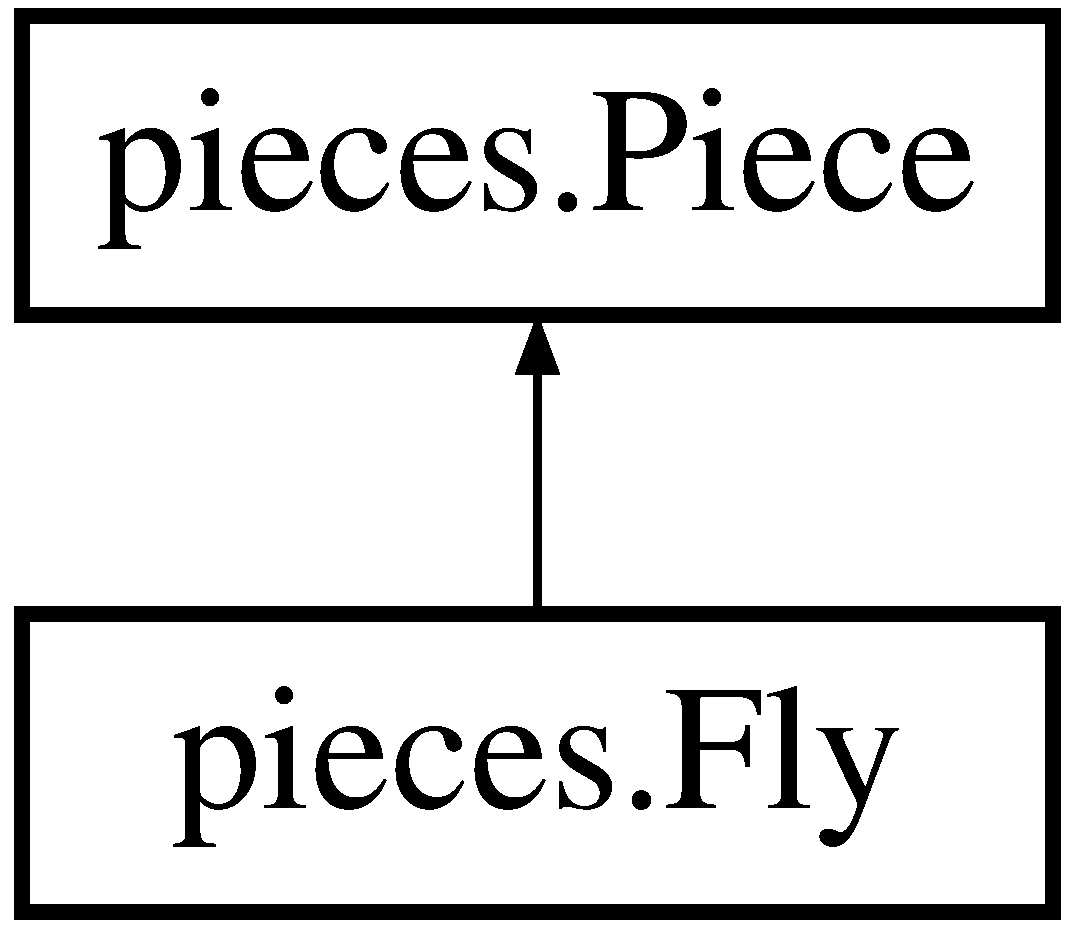
\includegraphics[height=2.000000cm]{classpieces_1_1_fly}
\end{center}
\end{figure}
\subsection*{Public Member Functions}
\begin{DoxyCompactItemize}
\item 
\hyperlink{classpieces_1_1_fly_a90c1e86b5ead75232aeff42f5a7b4178}{Fly} (int \hyperlink{classpieces_1_1_piece_ae40d6201d0aed36f369dd9d8f55892e3}{piece\-Type}, Board my\-Board, int x, int y)
\item 
\hyperlink{classpieces_1_1_fly_affbd143fa129ce1c7a0017979576cd21}{Fly} (int \hyperlink{classpieces_1_1_piece_ae40d6201d0aed36f369dd9d8f55892e3}{piece\-Type})
\item 
boolean \hyperlink{classpieces_1_1_fly_a836ab8c05aa6120a14320f7cc9da6a0f}{can\-Move\-Between} (Position start, Position end)
\end{DoxyCompactItemize}
\subsection*{Additional Inherited Members}


\subsection{Constructor \& Destructor Documentation}
\hypertarget{classpieces_1_1_fly_a90c1e86b5ead75232aeff42f5a7b4178}{\index{pieces\-::\-Fly@{pieces\-::\-Fly}!Fly@{Fly}}
\index{Fly@{Fly}!pieces::Fly@{pieces\-::\-Fly}}
\subsubsection[{Fly}]{\setlength{\rightskip}{0pt plus 5cm}pieces.\-Fly.\-Fly (
\begin{DoxyParamCaption}
\item[{int}]{piece\-Type, }
\item[{Board}]{my\-Board, }
\item[{int}]{x, }
\item[{int}]{y}
\end{DoxyParamCaption}
)}}\label{classpieces_1_1_fly_a90c1e86b5ead75232aeff42f5a7b4178}
Constructor No check to verify if piece\-Type is a Archer. It is up to the caller to verify. \hypertarget{classpieces_1_1_fly_affbd143fa129ce1c7a0017979576cd21}{\index{pieces\-::\-Fly@{pieces\-::\-Fly}!Fly@{Fly}}
\index{Fly@{Fly}!pieces::Fly@{pieces\-::\-Fly}}
\subsubsection[{Fly}]{\setlength{\rightskip}{0pt plus 5cm}pieces.\-Fly.\-Fly (
\begin{DoxyParamCaption}
\item[{int}]{piece\-Type}
\end{DoxyParamCaption}
)}}\label{classpieces_1_1_fly_affbd143fa129ce1c7a0017979576cd21}
Constructor 

\subsection{Member Function Documentation}
\hypertarget{classpieces_1_1_fly_a836ab8c05aa6120a14320f7cc9da6a0f}{\index{pieces\-::\-Fly@{pieces\-::\-Fly}!can\-Move\-Between@{can\-Move\-Between}}
\index{can\-Move\-Between@{can\-Move\-Between}!pieces::Fly@{pieces\-::\-Fly}}
\subsubsection[{can\-Move\-Between}]{\setlength{\rightskip}{0pt plus 5cm}boolean pieces.\-Fly.\-can\-Move\-Between (
\begin{DoxyParamCaption}
\item[{Position}]{start, }
\item[{Position}]{end}
\end{DoxyParamCaption}
)}}\label{classpieces_1_1_fly_a836ab8c05aa6120a14320f7cc9da6a0f}
Check if the piece can move from start to end location. \begin{DoxyReturn}{Returns}
true if it can. false otherwise. 
\end{DoxyReturn}


The documentation for this class was generated from the following file\-:\begin{DoxyCompactItemize}
\item 
/\-Volumes/\-Shared/\-Dropbox/\-Fall 13/\-C\-S 242/workspace/\-Chess/pieces/\hyperlink{_fly_8java}{Fly.\-java}\end{DoxyCompactItemize}

\hypertarget{classpieces_1_1_fly_trap}{\section{pieces.\-Fly\-Trap Class Reference}
\label{classpieces_1_1_fly_trap}\index{pieces.\-Fly\-Trap@{pieces.\-Fly\-Trap}}
}
Inheritance diagram for pieces.\-Fly\-Trap\-:\begin{figure}[H]
\begin{center}
\leavevmode
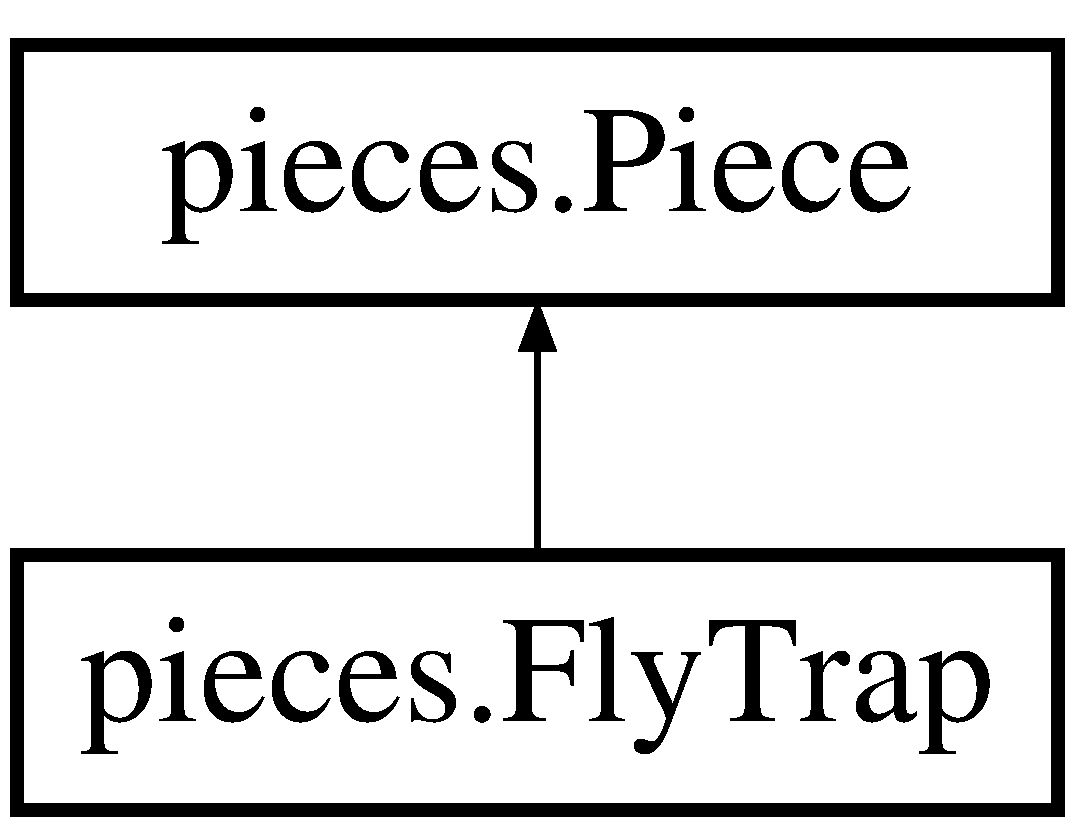
\includegraphics[height=2.000000cm]{classpieces_1_1_fly_trap}
\end{center}
\end{figure}
\subsection*{Public Member Functions}
\begin{DoxyCompactItemize}
\item 
\hyperlink{classpieces_1_1_fly_trap_aa8047ea9187379cf8aaa37773a5b53a0}{Fly\-Trap} (int \hyperlink{classpieces_1_1_piece_ae40d6201d0aed36f369dd9d8f55892e3}{piece\-Type}, Board my\-Board, int x, int y)
\item 
\hyperlink{classpieces_1_1_fly_trap_a699d7d74ce789d38aa3531d69c055537}{Fly\-Trap} (int \hyperlink{classpieces_1_1_piece_ae40d6201d0aed36f369dd9d8f55892e3}{piece\-Type})
\item 
boolean \hyperlink{classpieces_1_1_fly_trap_a36e41ba9c72806f3e93f7853270c0d41}{can\-Move\-Between} (Position start, Position end)
\end{DoxyCompactItemize}
\subsection*{Additional Inherited Members}


\subsection{Constructor \& Destructor Documentation}
\hypertarget{classpieces_1_1_fly_trap_aa8047ea9187379cf8aaa37773a5b53a0}{\index{pieces\-::\-Fly\-Trap@{pieces\-::\-Fly\-Trap}!Fly\-Trap@{Fly\-Trap}}
\index{Fly\-Trap@{Fly\-Trap}!pieces::FlyTrap@{pieces\-::\-Fly\-Trap}}
\subsubsection[{Fly\-Trap}]{\setlength{\rightskip}{0pt plus 5cm}pieces.\-Fly\-Trap.\-Fly\-Trap (
\begin{DoxyParamCaption}
\item[{int}]{piece\-Type, }
\item[{Board}]{my\-Board, }
\item[{int}]{x, }
\item[{int}]{y}
\end{DoxyParamCaption}
)}}\label{classpieces_1_1_fly_trap_aa8047ea9187379cf8aaa37773a5b53a0}
Constructor No check to verify if piece\-Type is a Peasant. It is up to the caller to verify. \hypertarget{classpieces_1_1_fly_trap_a699d7d74ce789d38aa3531d69c055537}{\index{pieces\-::\-Fly\-Trap@{pieces\-::\-Fly\-Trap}!Fly\-Trap@{Fly\-Trap}}
\index{Fly\-Trap@{Fly\-Trap}!pieces::FlyTrap@{pieces\-::\-Fly\-Trap}}
\subsubsection[{Fly\-Trap}]{\setlength{\rightskip}{0pt plus 5cm}pieces.\-Fly\-Trap.\-Fly\-Trap (
\begin{DoxyParamCaption}
\item[{int}]{piece\-Type}
\end{DoxyParamCaption}
)}}\label{classpieces_1_1_fly_trap_a699d7d74ce789d38aa3531d69c055537}
Constructor 

\subsection{Member Function Documentation}
\hypertarget{classpieces_1_1_fly_trap_a36e41ba9c72806f3e93f7853270c0d41}{\index{pieces\-::\-Fly\-Trap@{pieces\-::\-Fly\-Trap}!can\-Move\-Between@{can\-Move\-Between}}
\index{can\-Move\-Between@{can\-Move\-Between}!pieces::FlyTrap@{pieces\-::\-Fly\-Trap}}
\subsubsection[{can\-Move\-Between}]{\setlength{\rightskip}{0pt plus 5cm}boolean pieces.\-Fly\-Trap.\-can\-Move\-Between (
\begin{DoxyParamCaption}
\item[{Position}]{start, }
\item[{Position}]{end}
\end{DoxyParamCaption}
)}}\label{classpieces_1_1_fly_trap_a36e41ba9c72806f3e93f7853270c0d41}
Check if the piece can move from start to end location \begin{DoxyReturn}{Returns}
true if it can. false otherwise. 
\end{DoxyReturn}


The documentation for this class was generated from the following file\-:\begin{DoxyCompactItemize}
\item 
/\-Volumes/\-Shared/\-Dropbox/\-Fall 13/\-C\-S 242/workspace/\-Chess/pieces/\hyperlink{_fly_trap_8java}{Fly\-Trap.\-java}\end{DoxyCompactItemize}

\hypertarget{classgame_1_1_game}{\section{game.\-Game Class Reference}
\label{classgame_1_1_game}\index{game.\-Game@{game.\-Game}}
}
\subsection*{Classes}
\begin{DoxyCompactItemize}
\item 
class \hyperlink{classgame_1_1_game_1_1_state}{State}
\end{DoxyCompactItemize}
\subsection*{Public Member Functions}
\begin{DoxyCompactItemize}
\item 
\hyperlink{classgame_1_1_game_a901aa8c93a570f54854a9f08118a9451}{Game} ()
\item 
\hyperlink{classgame_1_1_game_aaefa1fc50584f2a2baf49974b704ae10}{Game} (int game\-Type)
\item 
void \hyperlink{classgame_1_1_game_ab6465ec6eafff324e0fc68ce665726ab}{new\-Game} (int game\-Type)
\item 
boolean \hyperlink{classgame_1_1_game_a08c47d9e26922ece9471182c46fe26f2}{select\-Move} (int x, int y)
\item 
boolean \hyperlink{classgame_1_1_game_a1d28d967b55b16467e07bf4b91bc274f}{move} (\hyperlink{classgame_1_1_position}{Position} start, \hyperlink{classgame_1_1_position}{Position} end)
\item 
boolean \hyperlink{classgame_1_1_game_a4c5b250a5732de27fef9f01d220e0932}{undo\-Move} ()
\item 
void \hyperlink{classgame_1_1_game_a828355cd26947a2473a273a1ff72d5ca}{update\-Board\-With\-Move} (\hyperlink{classgame_1_1_position}{Position} start, \hyperlink{classgame_1_1_position}{Position} end)
\item 
boolean \hyperlink{classgame_1_1_game_a7addda3056ed9f058c2c43c39d0db266}{is\-Check\-For} (int color)
\item 
boolean \hyperlink{classgame_1_1_game_a12eeb8d6a4b495aa0119aaaf6f3a1fd0}{is\-Checkmate\-For} (int color)
\item 
void \hyperlink{classgame_1_1_game_a0b0bcb102480072383c993fe21a2f788}{next\-Turn} ()
\item 
boolean \hyperlink{classgame_1_1_game_a1d7d7789913fc86cc195d49fbc61a4b4}{has\-Ended} ()
\item 
int \hyperlink{classgame_1_1_game_aad20d0a2c0db52757cdd44daf085396a}{get\-Winner} ()
\item 
boolean \hyperlink{classgame_1_1_game_a45abcf63801ae8a47951c840aebe6309}{player\-Put\-Self\-In\-Check} ()
\item 
\hyperlink{classgame_1_1_game_1_1_state}{State} \hyperlink{classgame_1_1_game_a0aab6da42b87bd5b3d5e86b2f3548ea3}{get\-Current\-State} ()
\end{DoxyCompactItemize}
\subsection*{Public Attributes}
\begin{DoxyCompactItemize}
\item 
\hyperlink{classgame_1_1_board}{Board} \hyperlink{classgame_1_1_game_a37e0047161981c19ff69a8cfdc633dd1}{board}
\end{DoxyCompactItemize}
\subsection*{Static Public Attributes}
\begin{DoxyCompactItemize}
\item 
static final int \hyperlink{classgame_1_1_game_a787b82f6054bed8334222d3aef9179e5}{E\-M\-P\-T\-Y} = 0
\item 
static final int \hyperlink{classgame_1_1_game_a8bca27c17a917044170e6d5d127736af}{C\-L\-A\-S\-S\-I\-C} = 1
\item 
static final int \hyperlink{classgame_1_1_game_a3b51812195a43b53c46afc14482e5d7b}{C\-U\-S\-T\-O\-M} = 2
\item 
static final int \hyperlink{classgame_1_1_game_ac15f5930449e1e16d9b7d4dd10b9c957}{W\-H\-I\-T\-E} = 1
\item 
static final int \hyperlink{classgame_1_1_game_a64750fe2b8cab1a3c14015732368118c}{B\-L\-A\-C\-K} = -\/1
\end{DoxyCompactItemize}
\subsection*{Private Attributes}
\begin{DoxyCompactItemize}
\item 
\hyperlink{classgame_1_1_game_1_1_state}{State} \hyperlink{classgame_1_1_game_a59957adcd9db3f8c3a9cda28729c881d}{current\-State}
\item 
int \hyperlink{classgame_1_1_game_aa55030dc8792bb216e934ca6a7d389fb}{winner}
\end{DoxyCompactItemize}


\subsection{Constructor \& Destructor Documentation}
\hypertarget{classgame_1_1_game_a901aa8c93a570f54854a9f08118a9451}{\index{game\-::\-Game@{game\-::\-Game}!Game@{Game}}
\index{Game@{Game}!game::Game@{game\-::\-Game}}
\subsubsection[{Game}]{\setlength{\rightskip}{0pt plus 5cm}game.\-Game.\-Game (
\begin{DoxyParamCaption}
{}
\end{DoxyParamCaption}
)}}\label{classgame_1_1_game_a901aa8c93a570f54854a9f08118a9451}
Constructor. \hypertarget{classgame_1_1_game_aaefa1fc50584f2a2baf49974b704ae10}{\index{game\-::\-Game@{game\-::\-Game}!Game@{Game}}
\index{Game@{Game}!game::Game@{game\-::\-Game}}
\subsubsection[{Game}]{\setlength{\rightskip}{0pt plus 5cm}game.\-Game.\-Game (
\begin{DoxyParamCaption}
\item[{int}]{game\-Type}
\end{DoxyParamCaption}
)}}\label{classgame_1_1_game_aaefa1fc50584f2a2baf49974b704ae10}
Constructor to start a new game. 
\begin{DoxyParams}{Parameters}
{\em game\-Type} & \\
\hline
\end{DoxyParams}


\subsection{Member Function Documentation}
\hypertarget{classgame_1_1_game_a0aab6da42b87bd5b3d5e86b2f3548ea3}{\index{game\-::\-Game@{game\-::\-Game}!get\-Current\-State@{get\-Current\-State}}
\index{get\-Current\-State@{get\-Current\-State}!game::Game@{game\-::\-Game}}
\subsubsection[{get\-Current\-State}]{\setlength{\rightskip}{0pt plus 5cm}{\bf State} game.\-Game.\-get\-Current\-State (
\begin{DoxyParamCaption}
{}
\end{DoxyParamCaption}
)}}\label{classgame_1_1_game_a0aab6da42b87bd5b3d5e86b2f3548ea3}
\hypertarget{classgame_1_1_game_aad20d0a2c0db52757cdd44daf085396a}{\index{game\-::\-Game@{game\-::\-Game}!get\-Winner@{get\-Winner}}
\index{get\-Winner@{get\-Winner}!game::Game@{game\-::\-Game}}
\subsubsection[{get\-Winner}]{\setlength{\rightskip}{0pt plus 5cm}int game.\-Game.\-get\-Winner (
\begin{DoxyParamCaption}
{}
\end{DoxyParamCaption}
)}}\label{classgame_1_1_game_aad20d0a2c0db52757cdd44daf085396a}
Gets the winning color of the game \begin{DoxyReturn}{Returns}
Winning color. 0 is game has not ended. 
\end{DoxyReturn}
\hypertarget{classgame_1_1_game_a1d7d7789913fc86cc195d49fbc61a4b4}{\index{game\-::\-Game@{game\-::\-Game}!has\-Ended@{has\-Ended}}
\index{has\-Ended@{has\-Ended}!game::Game@{game\-::\-Game}}
\subsubsection[{has\-Ended}]{\setlength{\rightskip}{0pt plus 5cm}boolean game.\-Game.\-has\-Ended (
\begin{DoxyParamCaption}
{}
\end{DoxyParamCaption}
)}}\label{classgame_1_1_game_a1d7d7789913fc86cc195d49fbc61a4b4}
Checks if the game has ended. \begin{DoxyReturn}{Returns}
True if it has ended. False otherwise. 
\end{DoxyReturn}
\hypertarget{classgame_1_1_game_a7addda3056ed9f058c2c43c39d0db266}{\index{game\-::\-Game@{game\-::\-Game}!is\-Check\-For@{is\-Check\-For}}
\index{is\-Check\-For@{is\-Check\-For}!game::Game@{game\-::\-Game}}
\subsubsection[{is\-Check\-For}]{\setlength{\rightskip}{0pt plus 5cm}boolean game.\-Game.\-is\-Check\-For (
\begin{DoxyParamCaption}
\item[{int}]{color}
\end{DoxyParamCaption}
)}}\label{classgame_1_1_game_a7addda3056ed9f058c2c43c39d0db266}
Checks if the player's king is in check \begin{DoxyReturn}{Returns}
True player is in check, false otherwise 
\end{DoxyReturn}
\hypertarget{classgame_1_1_game_a12eeb8d6a4b495aa0119aaaf6f3a1fd0}{\index{game\-::\-Game@{game\-::\-Game}!is\-Checkmate\-For@{is\-Checkmate\-For}}
\index{is\-Checkmate\-For@{is\-Checkmate\-For}!game::Game@{game\-::\-Game}}
\subsubsection[{is\-Checkmate\-For}]{\setlength{\rightskip}{0pt plus 5cm}boolean game.\-Game.\-is\-Checkmate\-For (
\begin{DoxyParamCaption}
\item[{int}]{color}
\end{DoxyParamCaption}
)}}\label{classgame_1_1_game_a12eeb8d6a4b495aa0119aaaf6f3a1fd0}
Checks if the player's king is in check \begin{DoxyReturn}{Returns}
True player is in check, false otherwise 
\end{DoxyReturn}
\hypertarget{classgame_1_1_game_a1d28d967b55b16467e07bf4b91bc274f}{\index{game\-::\-Game@{game\-::\-Game}!move@{move}}
\index{move@{move}!game::Game@{game\-::\-Game}}
\subsubsection[{move}]{\setlength{\rightskip}{0pt plus 5cm}boolean game.\-Game.\-move (
\begin{DoxyParamCaption}
\item[{{\bf Position}}]{start, }
\item[{{\bf Position}}]{end}
\end{DoxyParamCaption}
)}}\label{classgame_1_1_game_a1d28d967b55b16467e07bf4b91bc274f}
Tries to move a piece from start to end position  start and end must be on the board. 
\begin{DoxyParams}{Parameters}
{\em start} & and end positions, and the board object \\
\hline
\end{DoxyParams}
\begin{DoxyReturn}{Returns}
true on successful move, false on failure. 
\end{DoxyReturn}
\hypertarget{classgame_1_1_game_ab6465ec6eafff324e0fc68ce665726ab}{\index{game\-::\-Game@{game\-::\-Game}!new\-Game@{new\-Game}}
\index{new\-Game@{new\-Game}!game::Game@{game\-::\-Game}}
\subsubsection[{new\-Game}]{\setlength{\rightskip}{0pt plus 5cm}void game.\-Game.\-new\-Game (
\begin{DoxyParamCaption}
\item[{int}]{game\-Type}
\end{DoxyParamCaption}
)}}\label{classgame_1_1_game_ab6465ec6eafff324e0fc68ce665726ab}
Starts a new game from a constructor or after one has been called. 
\begin{DoxyParams}{Parameters}
{\em game\-Type} & \\
\hline
\end{DoxyParams}
\hypertarget{classgame_1_1_game_a0b0bcb102480072383c993fe21a2f788}{\index{game\-::\-Game@{game\-::\-Game}!next\-Turn@{next\-Turn}}
\index{next\-Turn@{next\-Turn}!game::Game@{game\-::\-Game}}
\subsubsection[{next\-Turn}]{\setlength{\rightskip}{0pt plus 5cm}void game.\-Game.\-next\-Turn (
\begin{DoxyParamCaption}
{}
\end{DoxyParamCaption}
)}}\label{classgame_1_1_game_a0b0bcb102480072383c993fe21a2f788}
Changes turns \hypertarget{classgame_1_1_game_a45abcf63801ae8a47951c840aebe6309}{\index{game\-::\-Game@{game\-::\-Game}!player\-Put\-Self\-In\-Check@{player\-Put\-Self\-In\-Check}}
\index{player\-Put\-Self\-In\-Check@{player\-Put\-Self\-In\-Check}!game::Game@{game\-::\-Game}}
\subsubsection[{player\-Put\-Self\-In\-Check}]{\setlength{\rightskip}{0pt plus 5cm}boolean game.\-Game.\-player\-Put\-Self\-In\-Check (
\begin{DoxyParamCaption}
{}
\end{DoxyParamCaption}
)}}\label{classgame_1_1_game_a45abcf63801ae8a47951c840aebe6309}
\hypertarget{classgame_1_1_game_a08c47d9e26922ece9471182c46fe26f2}{\index{game\-::\-Game@{game\-::\-Game}!select\-Move@{select\-Move}}
\index{select\-Move@{select\-Move}!game::Game@{game\-::\-Game}}
\subsubsection[{select\-Move}]{\setlength{\rightskip}{0pt plus 5cm}boolean game.\-Game.\-select\-Move (
\begin{DoxyParamCaption}
\item[{int}]{x, }
\item[{int}]{y}
\end{DoxyParamCaption}
)}}\label{classgame_1_1_game_a08c47d9e26922ece9471182c46fe26f2}
Make moves by selecting one position at a time. First call to this function must be made by white with coordinates for a white piece. 
\begin{DoxyParams}{Parameters}
{\em x} & coordinate on the board \\
\hline
{\em y} & coordinate \\
\hline
\end{DoxyParams}
\begin{DoxyReturn}{Returns}
True if space can be selected. False otherwise. 
\end{DoxyReturn}
\hypertarget{classgame_1_1_game_a4c5b250a5732de27fef9f01d220e0932}{\index{game\-::\-Game@{game\-::\-Game}!undo\-Move@{undo\-Move}}
\index{undo\-Move@{undo\-Move}!game::Game@{game\-::\-Game}}
\subsubsection[{undo\-Move}]{\setlength{\rightskip}{0pt plus 5cm}boolean game.\-Game.\-undo\-Move (
\begin{DoxyParamCaption}
{}
\end{DoxyParamCaption}
)}}\label{classgame_1_1_game_a4c5b250a5732de27fef9f01d220e0932}
Undoes move if possible \hypertarget{classgame_1_1_game_a828355cd26947a2473a273a1ff72d5ca}{\index{game\-::\-Game@{game\-::\-Game}!update\-Board\-With\-Move@{update\-Board\-With\-Move}}
\index{update\-Board\-With\-Move@{update\-Board\-With\-Move}!game::Game@{game\-::\-Game}}
\subsubsection[{update\-Board\-With\-Move}]{\setlength{\rightskip}{0pt plus 5cm}void game.\-Game.\-update\-Board\-With\-Move (
\begin{DoxyParamCaption}
\item[{{\bf Position}}]{start, }
\item[{{\bf Position}}]{end}
\end{DoxyParamCaption}
)}}\label{classgame_1_1_game_a828355cd26947a2473a273a1ff72d5ca}
Removes piece from start and puts it in end. Start is set to null. Should only be called from Mover class. 

\subsection{Member Data Documentation}
\hypertarget{classgame_1_1_game_a64750fe2b8cab1a3c14015732368118c}{\index{game\-::\-Game@{game\-::\-Game}!B\-L\-A\-C\-K@{B\-L\-A\-C\-K}}
\index{B\-L\-A\-C\-K@{B\-L\-A\-C\-K}!game::Game@{game\-::\-Game}}
\subsubsection[{B\-L\-A\-C\-K}]{\setlength{\rightskip}{0pt plus 5cm}final int game.\-Game.\-B\-L\-A\-C\-K = -\/1\hspace{0.3cm}{\ttfamily [static]}}}\label{classgame_1_1_game_a64750fe2b8cab1a3c14015732368118c}
\hypertarget{classgame_1_1_game_a37e0047161981c19ff69a8cfdc633dd1}{\index{game\-::\-Game@{game\-::\-Game}!board@{board}}
\index{board@{board}!game::Game@{game\-::\-Game}}
\subsubsection[{board}]{\setlength{\rightskip}{0pt plus 5cm}{\bf Board} game.\-Game.\-board}}\label{classgame_1_1_game_a37e0047161981c19ff69a8cfdc633dd1}
\hypertarget{classgame_1_1_game_a8bca27c17a917044170e6d5d127736af}{\index{game\-::\-Game@{game\-::\-Game}!C\-L\-A\-S\-S\-I\-C@{C\-L\-A\-S\-S\-I\-C}}
\index{C\-L\-A\-S\-S\-I\-C@{C\-L\-A\-S\-S\-I\-C}!game::Game@{game\-::\-Game}}
\subsubsection[{C\-L\-A\-S\-S\-I\-C}]{\setlength{\rightskip}{0pt plus 5cm}final int game.\-Game.\-C\-L\-A\-S\-S\-I\-C = 1\hspace{0.3cm}{\ttfamily [static]}}}\label{classgame_1_1_game_a8bca27c17a917044170e6d5d127736af}
\hypertarget{classgame_1_1_game_a59957adcd9db3f8c3a9cda28729c881d}{\index{game\-::\-Game@{game\-::\-Game}!current\-State@{current\-State}}
\index{current\-State@{current\-State}!game::Game@{game\-::\-Game}}
\subsubsection[{current\-State}]{\setlength{\rightskip}{0pt plus 5cm}{\bf State} game.\-Game.\-current\-State\hspace{0.3cm}{\ttfamily [private]}}}\label{classgame_1_1_game_a59957adcd9db3f8c3a9cda28729c881d}
\hypertarget{classgame_1_1_game_a3b51812195a43b53c46afc14482e5d7b}{\index{game\-::\-Game@{game\-::\-Game}!C\-U\-S\-T\-O\-M@{C\-U\-S\-T\-O\-M}}
\index{C\-U\-S\-T\-O\-M@{C\-U\-S\-T\-O\-M}!game::Game@{game\-::\-Game}}
\subsubsection[{C\-U\-S\-T\-O\-M}]{\setlength{\rightskip}{0pt plus 5cm}final int game.\-Game.\-C\-U\-S\-T\-O\-M = 2\hspace{0.3cm}{\ttfamily [static]}}}\label{classgame_1_1_game_a3b51812195a43b53c46afc14482e5d7b}
\hypertarget{classgame_1_1_game_a787b82f6054bed8334222d3aef9179e5}{\index{game\-::\-Game@{game\-::\-Game}!E\-M\-P\-T\-Y@{E\-M\-P\-T\-Y}}
\index{E\-M\-P\-T\-Y@{E\-M\-P\-T\-Y}!game::Game@{game\-::\-Game}}
\subsubsection[{E\-M\-P\-T\-Y}]{\setlength{\rightskip}{0pt plus 5cm}final int game.\-Game.\-E\-M\-P\-T\-Y = 0\hspace{0.3cm}{\ttfamily [static]}}}\label{classgame_1_1_game_a787b82f6054bed8334222d3aef9179e5}
\hypertarget{classgame_1_1_game_ac15f5930449e1e16d9b7d4dd10b9c957}{\index{game\-::\-Game@{game\-::\-Game}!W\-H\-I\-T\-E@{W\-H\-I\-T\-E}}
\index{W\-H\-I\-T\-E@{W\-H\-I\-T\-E}!game::Game@{game\-::\-Game}}
\subsubsection[{W\-H\-I\-T\-E}]{\setlength{\rightskip}{0pt plus 5cm}final int game.\-Game.\-W\-H\-I\-T\-E = 1\hspace{0.3cm}{\ttfamily [static]}}}\label{classgame_1_1_game_ac15f5930449e1e16d9b7d4dd10b9c957}
\hypertarget{classgame_1_1_game_aa55030dc8792bb216e934ca6a7d389fb}{\index{game\-::\-Game@{game\-::\-Game}!winner@{winner}}
\index{winner@{winner}!game::Game@{game\-::\-Game}}
\subsubsection[{winner}]{\setlength{\rightskip}{0pt plus 5cm}int game.\-Game.\-winner\hspace{0.3cm}{\ttfamily [private]}}}\label{classgame_1_1_game_aa55030dc8792bb216e934ca6a7d389fb}


The documentation for this class was generated from the following file\-:\begin{DoxyCompactItemize}
\item 
/\-Volumes/\-Shared/\-Dropbox/\-Fall 13/\-C\-S 242/workspace/\-Chess/game/\hyperlink{_game_8java}{Game.\-java}\end{DoxyCompactItemize}

\hypertarget{classpieces_1_1_king}{\section{pieces.\-King Class Reference}
\label{classpieces_1_1_king}\index{pieces.\-King@{pieces.\-King}}
}
Inheritance diagram for pieces.\-King\-:\begin{figure}[H]
\begin{center}
\leavevmode
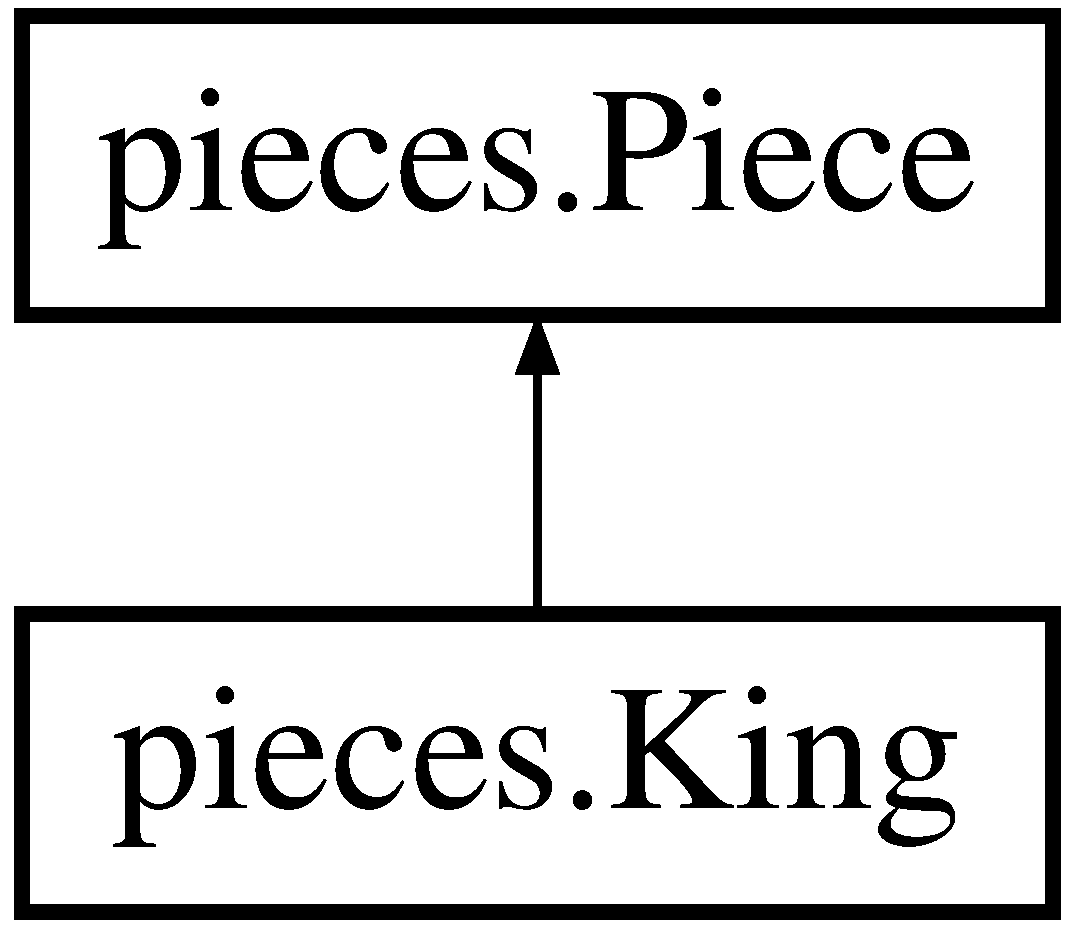
\includegraphics[height=2.000000cm]{classpieces_1_1_king}
\end{center}
\end{figure}
\subsection*{Public Member Functions}
\begin{DoxyCompactItemize}
\item 
\hyperlink{classpieces_1_1_king_a684c747c60fc259009d31bc181207684}{King} (int \hyperlink{classpieces_1_1_piece_ae40d6201d0aed36f369dd9d8f55892e3}{piece\-Type}, Board my\-Board, int x, int y)
\item 
\hyperlink{classpieces_1_1_king_a3aae06954339042f484172df9cccbece}{King} (int \hyperlink{classpieces_1_1_piece_ae40d6201d0aed36f369dd9d8f55892e3}{piece\-Type})
\item 
boolean \hyperlink{classpieces_1_1_king_a856cf67c82dd9f19d0aec479677c9260}{can\-Move\-Between} (Position start, Position end)
\end{DoxyCompactItemize}
\subsection*{Additional Inherited Members}


\subsection{Constructor \& Destructor Documentation}
\hypertarget{classpieces_1_1_king_a684c747c60fc259009d31bc181207684}{\index{pieces\-::\-King@{pieces\-::\-King}!King@{King}}
\index{King@{King}!pieces::King@{pieces\-::\-King}}
\subsubsection[{King}]{\setlength{\rightskip}{0pt plus 5cm}pieces.\-King.\-King (
\begin{DoxyParamCaption}
\item[{int}]{piece\-Type, }
\item[{Board}]{my\-Board, }
\item[{int}]{x, }
\item[{int}]{y}
\end{DoxyParamCaption}
)}}\label{classpieces_1_1_king_a684c747c60fc259009d31bc181207684}
Constructor No check to verify if piece\-Type is a \hyperlink{classpieces_1_1_king}{King}. It is up to the caller to verify. \hypertarget{classpieces_1_1_king_a3aae06954339042f484172df9cccbece}{\index{pieces\-::\-King@{pieces\-::\-King}!King@{King}}
\index{King@{King}!pieces::King@{pieces\-::\-King}}
\subsubsection[{King}]{\setlength{\rightskip}{0pt plus 5cm}pieces.\-King.\-King (
\begin{DoxyParamCaption}
\item[{int}]{piece\-Type}
\end{DoxyParamCaption}
)}}\label{classpieces_1_1_king_a3aae06954339042f484172df9cccbece}
Constructor 

\subsection{Member Function Documentation}
\hypertarget{classpieces_1_1_king_a856cf67c82dd9f19d0aec479677c9260}{\index{pieces\-::\-King@{pieces\-::\-King}!can\-Move\-Between@{can\-Move\-Between}}
\index{can\-Move\-Between@{can\-Move\-Between}!pieces::King@{pieces\-::\-King}}
\subsubsection[{can\-Move\-Between}]{\setlength{\rightskip}{0pt plus 5cm}boolean pieces.\-King.\-can\-Move\-Between (
\begin{DoxyParamCaption}
\item[{Position}]{start, }
\item[{Position}]{end}
\end{DoxyParamCaption}
)}}\label{classpieces_1_1_king_a856cf67c82dd9f19d0aec479677c9260}
Check if the piece can move from start to end location \begin{DoxyReturn}{Returns}
true if it can. false otherwise. 
\end{DoxyReturn}


The documentation for this class was generated from the following file\-:\begin{DoxyCompactItemize}
\item 
/\-Volumes/\-Shared/\-Dropbox/\-Fall 13/\-C\-S 242/workspace/\-Chess/pieces/\hyperlink{_king_8java}{King.\-java}\end{DoxyCompactItemize}

\hypertarget{classpieces_1_1_knight}{\section{pieces.\-Knight Class Reference}
\label{classpieces_1_1_knight}\index{pieces.\-Knight@{pieces.\-Knight}}
}
Inheritance diagram for pieces.\-Knight\-:\begin{figure}[H]
\begin{center}
\leavevmode
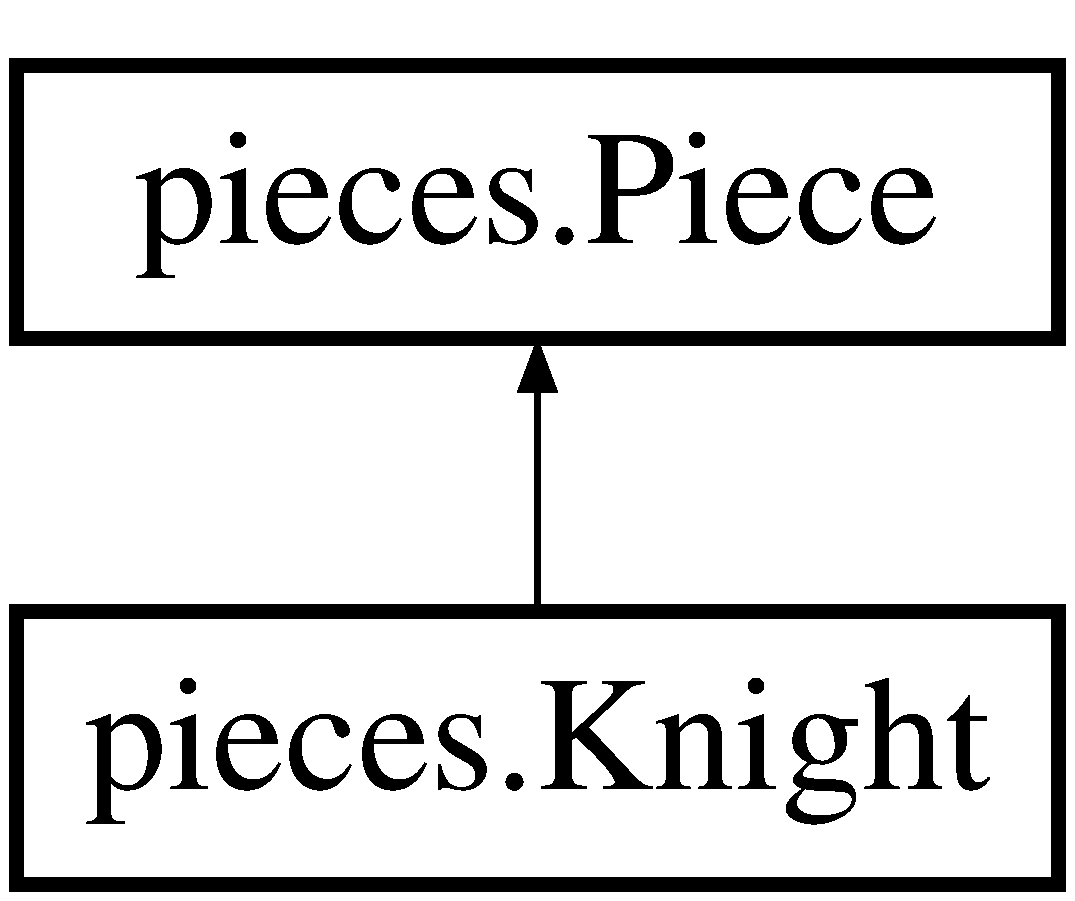
\includegraphics[height=2.000000cm]{classpieces_1_1_knight}
\end{center}
\end{figure}
\subsection*{Public Member Functions}
\begin{DoxyCompactItemize}
\item 
\hyperlink{classpieces_1_1_knight_ae733eecc6297202b8430d391941c6ef9}{Knight} (int \hyperlink{classpieces_1_1_piece_ae40d6201d0aed36f369dd9d8f55892e3}{piece\-Type}, Board my\-Board, int x, int y)
\item 
\hyperlink{classpieces_1_1_knight_abbd52d0308ba15b0a68ce3270c536991}{Knight} (int \hyperlink{classpieces_1_1_piece_ae40d6201d0aed36f369dd9d8f55892e3}{piece\-Type})
\item 
boolean \hyperlink{classpieces_1_1_knight_ae71c97f71f48ceb3301667eda116506f}{can\-Move\-Between} (Position start, Position end)
\end{DoxyCompactItemize}
\subsection*{Additional Inherited Members}


\subsection{Constructor \& Destructor Documentation}
\hypertarget{classpieces_1_1_knight_ae733eecc6297202b8430d391941c6ef9}{\index{pieces\-::\-Knight@{pieces\-::\-Knight}!Knight@{Knight}}
\index{Knight@{Knight}!pieces::Knight@{pieces\-::\-Knight}}
\subsubsection[{Knight}]{\setlength{\rightskip}{0pt plus 5cm}pieces.\-Knight.\-Knight (
\begin{DoxyParamCaption}
\item[{int}]{piece\-Type, }
\item[{Board}]{my\-Board, }
\item[{int}]{x, }
\item[{int}]{y}
\end{DoxyParamCaption}
)}}\label{classpieces_1_1_knight_ae733eecc6297202b8430d391941c6ef9}
Constructor No check to verify if piece\-Type is a \hyperlink{classpieces_1_1_knight}{Knight}. It is up to the caller to verify. \hypertarget{classpieces_1_1_knight_abbd52d0308ba15b0a68ce3270c536991}{\index{pieces\-::\-Knight@{pieces\-::\-Knight}!Knight@{Knight}}
\index{Knight@{Knight}!pieces::Knight@{pieces\-::\-Knight}}
\subsubsection[{Knight}]{\setlength{\rightskip}{0pt plus 5cm}pieces.\-Knight.\-Knight (
\begin{DoxyParamCaption}
\item[{int}]{piece\-Type}
\end{DoxyParamCaption}
)}}\label{classpieces_1_1_knight_abbd52d0308ba15b0a68ce3270c536991}
Constructor 

\subsection{Member Function Documentation}
\hypertarget{classpieces_1_1_knight_ae71c97f71f48ceb3301667eda116506f}{\index{pieces\-::\-Knight@{pieces\-::\-Knight}!can\-Move\-Between@{can\-Move\-Between}}
\index{can\-Move\-Between@{can\-Move\-Between}!pieces::Knight@{pieces\-::\-Knight}}
\subsubsection[{can\-Move\-Between}]{\setlength{\rightskip}{0pt plus 5cm}boolean pieces.\-Knight.\-can\-Move\-Between (
\begin{DoxyParamCaption}
\item[{Position}]{start, }
\item[{Position}]{end}
\end{DoxyParamCaption}
)}}\label{classpieces_1_1_knight_ae71c97f71f48ceb3301667eda116506f}
Check if the piece can move from start to end location. \begin{DoxyReturn}{Returns}
true if it can. false otherwise. 
\end{DoxyReturn}


The documentation for this class was generated from the following file\-:\begin{DoxyCompactItemize}
\item 
/\-Volumes/\-Shared/\-Dropbox/\-Fall 13/\-C\-S 242/workspace/\-Chess/pieces/\hyperlink{_knight_8java}{Knight.\-java}\end{DoxyCompactItemize}

\hypertarget{classpieces_1_1_pawn}{\section{pieces.\-Pawn Class Reference}
\label{classpieces_1_1_pawn}\index{pieces.\-Pawn@{pieces.\-Pawn}}
}
Inheritance diagram for pieces.\-Pawn\-:\begin{figure}[H]
\begin{center}
\leavevmode
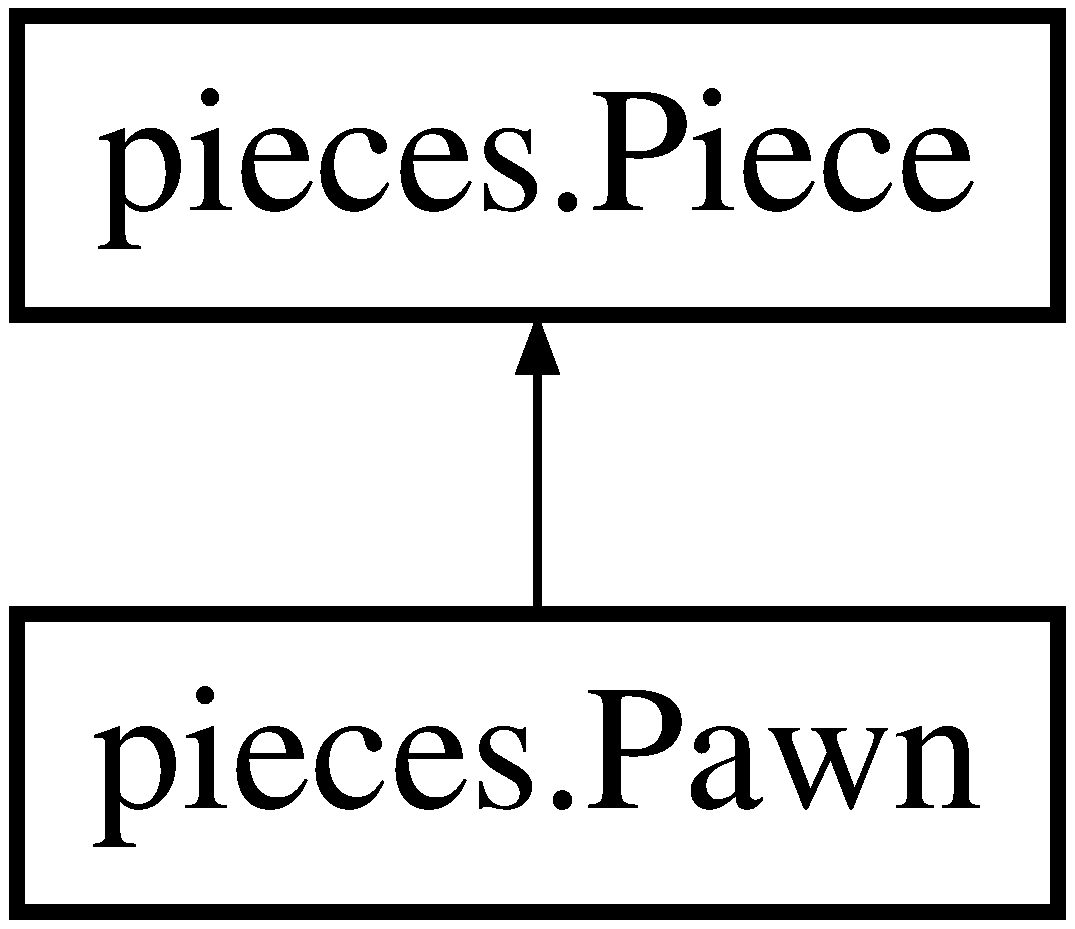
\includegraphics[height=2.000000cm]{classpieces_1_1_pawn}
\end{center}
\end{figure}
\subsection*{Public Member Functions}
\begin{DoxyCompactItemize}
\item 
\hyperlink{classpieces_1_1_pawn_afba214edbf76842349a8081436d65905}{Pawn} (int \hyperlink{classpieces_1_1_piece_ae40d6201d0aed36f369dd9d8f55892e3}{piece\-Type}, Board my\-Board, int x, int y)
\item 
\hyperlink{classpieces_1_1_pawn_adb247ab1ea60ba83ced124ce94776180}{Pawn} (int \hyperlink{classpieces_1_1_piece_ae40d6201d0aed36f369dd9d8f55892e3}{piece\-Type})
\item 
boolean \hyperlink{classpieces_1_1_pawn_a1786e32a231e36a9f68e5c55b5e957a0}{can\-Move\-Between} (Position start, Position end)
\item 
boolean \hyperlink{classpieces_1_1_pawn_ae977b1dff93961350fe4130639bc83f3}{is\-Pawn\-Move} (Position start, Position end, Board board)
\end{DoxyCompactItemize}
\subsection*{Additional Inherited Members}


\subsection{Constructor \& Destructor Documentation}
\hypertarget{classpieces_1_1_pawn_afba214edbf76842349a8081436d65905}{\index{pieces\-::\-Pawn@{pieces\-::\-Pawn}!Pawn@{Pawn}}
\index{Pawn@{Pawn}!pieces::Pawn@{pieces\-::\-Pawn}}
\subsubsection[{Pawn}]{\setlength{\rightskip}{0pt plus 5cm}pieces.\-Pawn.\-Pawn (
\begin{DoxyParamCaption}
\item[{int}]{piece\-Type, }
\item[{Board}]{my\-Board, }
\item[{int}]{x, }
\item[{int}]{y}
\end{DoxyParamCaption}
)}}\label{classpieces_1_1_pawn_afba214edbf76842349a8081436d65905}
Constructor No check to verify if piece\-Type is a pawn. It is up to the caller to verify. \hypertarget{classpieces_1_1_pawn_adb247ab1ea60ba83ced124ce94776180}{\index{pieces\-::\-Pawn@{pieces\-::\-Pawn}!Pawn@{Pawn}}
\index{Pawn@{Pawn}!pieces::Pawn@{pieces\-::\-Pawn}}
\subsubsection[{Pawn}]{\setlength{\rightskip}{0pt plus 5cm}pieces.\-Pawn.\-Pawn (
\begin{DoxyParamCaption}
\item[{int}]{piece\-Type}
\end{DoxyParamCaption}
)}}\label{classpieces_1_1_pawn_adb247ab1ea60ba83ced124ce94776180}
Constructor 

\subsection{Member Function Documentation}
\hypertarget{classpieces_1_1_pawn_a1786e32a231e36a9f68e5c55b5e957a0}{\index{pieces\-::\-Pawn@{pieces\-::\-Pawn}!can\-Move\-Between@{can\-Move\-Between}}
\index{can\-Move\-Between@{can\-Move\-Between}!pieces::Pawn@{pieces\-::\-Pawn}}
\subsubsection[{can\-Move\-Between}]{\setlength{\rightskip}{0pt plus 5cm}boolean pieces.\-Pawn.\-can\-Move\-Between (
\begin{DoxyParamCaption}
\item[{Position}]{start, }
\item[{Position}]{end}
\end{DoxyParamCaption}
)}}\label{classpieces_1_1_pawn_a1786e32a231e36a9f68e5c55b5e957a0}
Check if the piece can move from start to end location. \begin{DoxyReturn}{Returns}
true if it can. false otherwise. 
\end{DoxyReturn}
\hypertarget{classpieces_1_1_pawn_ae977b1dff93961350fe4130639bc83f3}{\index{pieces\-::\-Pawn@{pieces\-::\-Pawn}!is\-Pawn\-Move@{is\-Pawn\-Move}}
\index{is\-Pawn\-Move@{is\-Pawn\-Move}!pieces::Pawn@{pieces\-::\-Pawn}}
\subsubsection[{is\-Pawn\-Move}]{\setlength{\rightskip}{0pt plus 5cm}boolean pieces.\-Pawn.\-is\-Pawn\-Move (
\begin{DoxyParamCaption}
\item[{Position}]{start, }
\item[{Position}]{end, }
\item[{Board}]{board}
\end{DoxyParamCaption}
)}}\label{classpieces_1_1_pawn_ae977b1dff93961350fe4130639bc83f3}
Checks if pawn is moving in the right direction and returns the number of ranks changed \begin{DoxyReturn}{Returns}
-\/1 if not moving ahead, number of ranks moving otherwise (including 0) 
\end{DoxyReturn}


The documentation for this class was generated from the following file\-:\begin{DoxyCompactItemize}
\item 
/\-Volumes/\-Shared/\-Dropbox/\-Fall 13/\-C\-S 242/workspace/\-Chess/pieces/\hyperlink{_pawn_8java}{Pawn.\-java}\end{DoxyCompactItemize}

\hypertarget{classpieces_1_1_piece}{\section{pieces.\-Piece Class Reference}
\label{classpieces_1_1_piece}\index{pieces.\-Piece@{pieces.\-Piece}}
}
Inheritance diagram for pieces.\-Piece\-:\begin{figure}[H]
\begin{center}
\leavevmode
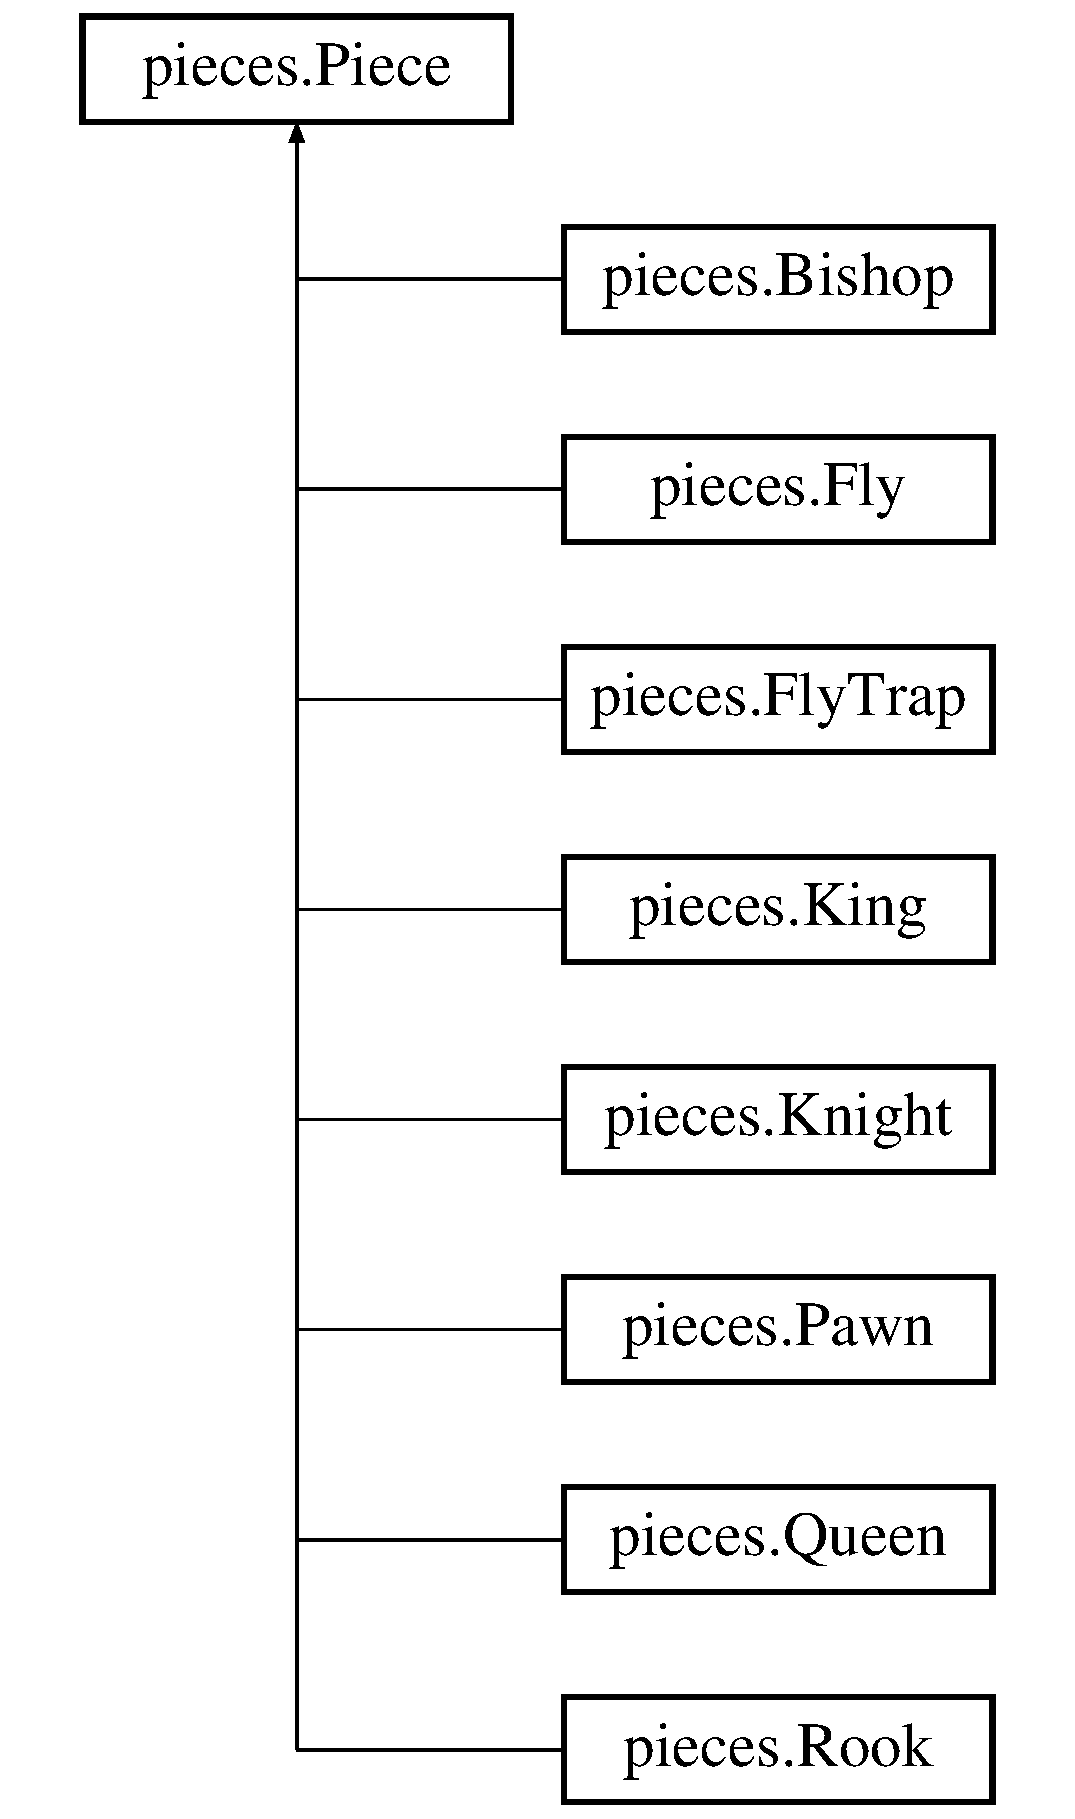
\includegraphics[height=9.000000cm]{classpieces_1_1_piece}
\end{center}
\end{figure}
\subsection*{Public Member Functions}
\begin{DoxyCompactItemize}
\item 
\hyperlink{classpieces_1_1_piece_a9f739de98fb95a5c379bddec6fa05a9f}{Piece} (int \hyperlink{classpieces_1_1_piece_ae40d6201d0aed36f369dd9d8f55892e3}{piece\-Type}, Board my\-Board, int x, int y)  throws Illegal\-Argument\-Exception
\item 
\hyperlink{classpieces_1_1_piece_a6cb26e7b2633c754553bf9e32d73f267}{Piece} (int \hyperlink{classpieces_1_1_piece_ae40d6201d0aed36f369dd9d8f55892e3}{piece\-Type})
\item 
boolean \hyperlink{classpieces_1_1_piece_a2217ef2be3a64bac127d9092f4ec4125}{can\-Move\-Between} (Position start, Position end)
\item 
int \hyperlink{classpieces_1_1_piece_a0a0c19217dbf20dc4b91b40798fb3083}{get\-Piece\-Type} ()
\item 
int \hyperlink{classpieces_1_1_piece_adfb40e69bb9e5a2f21a33a1e91682c44}{get\-Color} ()
\item 
Position \hyperlink{classpieces_1_1_piece_a74e034990e5f39e58ef48404102d65dd}{get\-Pos} ()
\item 
void \hyperlink{classpieces_1_1_piece_ac6422f94714df2fcddab8dc7a9372e4a}{set\-Pos} (Position \hyperlink{classpieces_1_1_piece_a9a3b5cf20c198c74a04cea615815b11c}{pos})
\item 
void \hyperlink{classpieces_1_1_piece_a3ac139a19545ca7736a850d4df5ad0c1}{set\-Board} (Board my\-Board)
\end{DoxyCompactItemize}
\subsection*{Static Public Attributes}
\begin{DoxyCompactItemize}
\item 
static int \hyperlink{classpieces_1_1_piece_a5d79a14b2b47d6699449dd3e015f0392}{E\-M\-P\-T\-Y} = 0
\item 
static int \hyperlink{classpieces_1_1_piece_a625b30e964a9962f2909525a6da66467}{P\-A\-W\-N} = 1
\item 
static int \hyperlink{classpieces_1_1_piece_abd3221f0cd505d49ca331c79264cb16f}{R\-O\-O\-K} = 2
\item 
static int \hyperlink{classpieces_1_1_piece_a594fad243368a3532079b3705fb18c00}{K\-N\-I\-G\-H\-T} = 3
\item 
static int \hyperlink{classpieces_1_1_piece_a61cc411a0431bb85a06365792d051a16}{B\-I\-S\-H\-O\-P} = 4
\item 
static int \hyperlink{classpieces_1_1_piece_a6bf04fb81c4004dbdf7ffe388d0d5709}{Q\-U\-E\-E\-N} = 5
\item 
static int \hyperlink{classpieces_1_1_piece_a21aac8b997842296b02cc95dc7caf482}{K\-I\-N\-G} = 6
\item 
static int \hyperlink{classpieces_1_1_piece_a63587ad284faac66495ede78b2c835d2}{A\-R\-C\-H\-E\-R} = 7
\item 
static int \hyperlink{classpieces_1_1_piece_a096ca129d441937377c6303f8a9b47dd}{P\-E\-A\-S\-A\-N\-T} = 8
\item 
static final int \hyperlink{classpieces_1_1_piece_a06ca63ba013da56fa10ccde66da622c7}{W\-H\-I\-T\-E} = 1
\item 
static final int \hyperlink{classpieces_1_1_piece_ab569c22ea0d43da6e1e9e1722b7f41b1}{B\-L\-A\-C\-K} = -\/1
\end{DoxyCompactItemize}
\subsection*{Protected Attributes}
\begin{DoxyCompactItemize}
\item 
int \hyperlink{classpieces_1_1_piece_a1ceedc99f8855c1fca9839aa5a69db69}{color}
\item 
int \hyperlink{classpieces_1_1_piece_ae40d6201d0aed36f369dd9d8f55892e3}{piece\-Type}
\item 
Position \hyperlink{classpieces_1_1_piece_a9a3b5cf20c198c74a04cea615815b11c}{pos}
\end{DoxyCompactItemize}


\subsection{Detailed Description}
An abstract class to represent a piece on the board. Each subclass must implement a unique can\-Move\-Between function \begin{DoxyAuthor}{Author}
Shashank Bharadwaj 
\end{DoxyAuthor}
\begin{DoxyDate}{Date}
Wed, 4 Sep 2013 
\end{DoxyDate}


\subsection{Constructor \& Destructor Documentation}
\hypertarget{classpieces_1_1_piece_a9f739de98fb95a5c379bddec6fa05a9f}{\index{pieces\-::\-Piece@{pieces\-::\-Piece}!Piece@{Piece}}
\index{Piece@{Piece}!pieces::Piece@{pieces\-::\-Piece}}
\subsubsection[{Piece}]{\setlength{\rightskip}{0pt plus 5cm}pieces.\-Piece.\-Piece (
\begin{DoxyParamCaption}
\item[{int}]{piece\-Type, }
\item[{Board}]{my\-Board, }
\item[{int}]{x, }
\item[{int}]{y}
\end{DoxyParamCaption}
) throws Illegal\-Argument\-Exception}}\label{classpieces_1_1_piece_a9f739de98fb95a5c379bddec6fa05a9f}
Constructs a \hyperlink{classpieces_1_1_piece}{Piece} with given type, color and position 
\begin{DoxyParams}{Parameters}
{\em piece\-Type,\-:} & Pieces numbered 1-\/6. Black -\/ and White + values \\
\hline
{\em my\-Board} & \\
\hline
{\em x,\-:} & coordinate \\
\hline
{\em y,\-:} & coordinate \\
\hline
\end{DoxyParams}
\hypertarget{classpieces_1_1_piece_a6cb26e7b2633c754553bf9e32d73f267}{\index{pieces\-::\-Piece@{pieces\-::\-Piece}!Piece@{Piece}}
\index{Piece@{Piece}!pieces::Piece@{pieces\-::\-Piece}}
\subsubsection[{Piece}]{\setlength{\rightskip}{0pt plus 5cm}pieces.\-Piece.\-Piece (
\begin{DoxyParamCaption}
\item[{int}]{piece\-Type}
\end{DoxyParamCaption}
)}}\label{classpieces_1_1_piece_a6cb26e7b2633c754553bf9e32d73f267}
Constructs a \hyperlink{classpieces_1_1_piece}{Piece} with given type and color 
\begin{DoxyParams}{Parameters}
{\em piece\-Type,\-:} & Pieces numbered 1-\/6. Black -\/ and White + values \\
\hline
{\em my\-Board} & \\
\hline
\end{DoxyParams}


\subsection{Member Function Documentation}
\hypertarget{classpieces_1_1_piece_a2217ef2be3a64bac127d9092f4ec4125}{\index{pieces\-::\-Piece@{pieces\-::\-Piece}!can\-Move\-Between@{can\-Move\-Between}}
\index{can\-Move\-Between@{can\-Move\-Between}!pieces::Piece@{pieces\-::\-Piece}}
\subsubsection[{can\-Move\-Between}]{\setlength{\rightskip}{0pt plus 5cm}boolean pieces.\-Piece.\-can\-Move\-Between (
\begin{DoxyParamCaption}
\item[{Position}]{start, }
\item[{Position}]{end}
\end{DoxyParamCaption}
)}}\label{classpieces_1_1_piece_a2217ef2be3a64bac127d9092f4ec4125}
Check if the piece can move from start to end location. Must be overridden in subclass. \begin{DoxyReturn}{Returns}
true if it can. false otherwise. 
\end{DoxyReturn}
\hypertarget{classpieces_1_1_piece_adfb40e69bb9e5a2f21a33a1e91682c44}{\index{pieces\-::\-Piece@{pieces\-::\-Piece}!get\-Color@{get\-Color}}
\index{get\-Color@{get\-Color}!pieces::Piece@{pieces\-::\-Piece}}
\subsubsection[{get\-Color}]{\setlength{\rightskip}{0pt plus 5cm}int pieces.\-Piece.\-get\-Color (
\begin{DoxyParamCaption}
{}
\end{DoxyParamCaption}
)}}\label{classpieces_1_1_piece_adfb40e69bb9e5a2f21a33a1e91682c44}
color getter \hypertarget{classpieces_1_1_piece_a0a0c19217dbf20dc4b91b40798fb3083}{\index{pieces\-::\-Piece@{pieces\-::\-Piece}!get\-Piece\-Type@{get\-Piece\-Type}}
\index{get\-Piece\-Type@{get\-Piece\-Type}!pieces::Piece@{pieces\-::\-Piece}}
\subsubsection[{get\-Piece\-Type}]{\setlength{\rightskip}{0pt plus 5cm}int pieces.\-Piece.\-get\-Piece\-Type (
\begin{DoxyParamCaption}
{}
\end{DoxyParamCaption}
)}}\label{classpieces_1_1_piece_a0a0c19217dbf20dc4b91b40798fb3083}
piece\-Type getter \hypertarget{classpieces_1_1_piece_a74e034990e5f39e58ef48404102d65dd}{\index{pieces\-::\-Piece@{pieces\-::\-Piece}!get\-Pos@{get\-Pos}}
\index{get\-Pos@{get\-Pos}!pieces::Piece@{pieces\-::\-Piece}}
\subsubsection[{get\-Pos}]{\setlength{\rightskip}{0pt plus 5cm}Position pieces.\-Piece.\-get\-Pos (
\begin{DoxyParamCaption}
{}
\end{DoxyParamCaption}
)}}\label{classpieces_1_1_piece_a74e034990e5f39e58ef48404102d65dd}
position getter \hypertarget{classpieces_1_1_piece_a3ac139a19545ca7736a850d4df5ad0c1}{\index{pieces\-::\-Piece@{pieces\-::\-Piece}!set\-Board@{set\-Board}}
\index{set\-Board@{set\-Board}!pieces::Piece@{pieces\-::\-Piece}}
\subsubsection[{set\-Board}]{\setlength{\rightskip}{0pt plus 5cm}void pieces.\-Piece.\-set\-Board (
\begin{DoxyParamCaption}
\item[{Board}]{my\-Board}
\end{DoxyParamCaption}
)}}\label{classpieces_1_1_piece_a3ac139a19545ca7736a850d4df5ad0c1}
position setter \hypertarget{classpieces_1_1_piece_ac6422f94714df2fcddab8dc7a9372e4a}{\index{pieces\-::\-Piece@{pieces\-::\-Piece}!set\-Pos@{set\-Pos}}
\index{set\-Pos@{set\-Pos}!pieces::Piece@{pieces\-::\-Piece}}
\subsubsection[{set\-Pos}]{\setlength{\rightskip}{0pt plus 5cm}void pieces.\-Piece.\-set\-Pos (
\begin{DoxyParamCaption}
\item[{Position}]{pos}
\end{DoxyParamCaption}
)}}\label{classpieces_1_1_piece_ac6422f94714df2fcddab8dc7a9372e4a}
position setter 

\subsection{Member Data Documentation}
\hypertarget{classpieces_1_1_piece_a63587ad284faac66495ede78b2c835d2}{\index{pieces\-::\-Piece@{pieces\-::\-Piece}!A\-R\-C\-H\-E\-R@{A\-R\-C\-H\-E\-R}}
\index{A\-R\-C\-H\-E\-R@{A\-R\-C\-H\-E\-R}!pieces::Piece@{pieces\-::\-Piece}}
\subsubsection[{A\-R\-C\-H\-E\-R}]{\setlength{\rightskip}{0pt plus 5cm}int pieces.\-Piece.\-A\-R\-C\-H\-E\-R = 7\hspace{0.3cm}{\ttfamily [static]}}}\label{classpieces_1_1_piece_a63587ad284faac66495ede78b2c835d2}
\hypertarget{classpieces_1_1_piece_a61cc411a0431bb85a06365792d051a16}{\index{pieces\-::\-Piece@{pieces\-::\-Piece}!B\-I\-S\-H\-O\-P@{B\-I\-S\-H\-O\-P}}
\index{B\-I\-S\-H\-O\-P@{B\-I\-S\-H\-O\-P}!pieces::Piece@{pieces\-::\-Piece}}
\subsubsection[{B\-I\-S\-H\-O\-P}]{\setlength{\rightskip}{0pt plus 5cm}int pieces.\-Piece.\-B\-I\-S\-H\-O\-P = 4\hspace{0.3cm}{\ttfamily [static]}}}\label{classpieces_1_1_piece_a61cc411a0431bb85a06365792d051a16}
\hypertarget{classpieces_1_1_piece_ab569c22ea0d43da6e1e9e1722b7f41b1}{\index{pieces\-::\-Piece@{pieces\-::\-Piece}!B\-L\-A\-C\-K@{B\-L\-A\-C\-K}}
\index{B\-L\-A\-C\-K@{B\-L\-A\-C\-K}!pieces::Piece@{pieces\-::\-Piece}}
\subsubsection[{B\-L\-A\-C\-K}]{\setlength{\rightskip}{0pt plus 5cm}final int pieces.\-Piece.\-B\-L\-A\-C\-K = -\/1\hspace{0.3cm}{\ttfamily [static]}}}\label{classpieces_1_1_piece_ab569c22ea0d43da6e1e9e1722b7f41b1}
\hypertarget{classpieces_1_1_piece_a1ceedc99f8855c1fca9839aa5a69db69}{\index{pieces\-::\-Piece@{pieces\-::\-Piece}!color@{color}}
\index{color@{color}!pieces::Piece@{pieces\-::\-Piece}}
\subsubsection[{color}]{\setlength{\rightskip}{0pt plus 5cm}int pieces.\-Piece.\-color\hspace{0.3cm}{\ttfamily [protected]}}}\label{classpieces_1_1_piece_a1ceedc99f8855c1fca9839aa5a69db69}
\hypertarget{classpieces_1_1_piece_a5d79a14b2b47d6699449dd3e015f0392}{\index{pieces\-::\-Piece@{pieces\-::\-Piece}!E\-M\-P\-T\-Y@{E\-M\-P\-T\-Y}}
\index{E\-M\-P\-T\-Y@{E\-M\-P\-T\-Y}!pieces::Piece@{pieces\-::\-Piece}}
\subsubsection[{E\-M\-P\-T\-Y}]{\setlength{\rightskip}{0pt plus 5cm}int pieces.\-Piece.\-E\-M\-P\-T\-Y = 0\hspace{0.3cm}{\ttfamily [static]}}}\label{classpieces_1_1_piece_a5d79a14b2b47d6699449dd3e015f0392}
\hypertarget{classpieces_1_1_piece_a21aac8b997842296b02cc95dc7caf482}{\index{pieces\-::\-Piece@{pieces\-::\-Piece}!K\-I\-N\-G@{K\-I\-N\-G}}
\index{K\-I\-N\-G@{K\-I\-N\-G}!pieces::Piece@{pieces\-::\-Piece}}
\subsubsection[{K\-I\-N\-G}]{\setlength{\rightskip}{0pt plus 5cm}int pieces.\-Piece.\-K\-I\-N\-G = 6\hspace{0.3cm}{\ttfamily [static]}}}\label{classpieces_1_1_piece_a21aac8b997842296b02cc95dc7caf482}
\hypertarget{classpieces_1_1_piece_a594fad243368a3532079b3705fb18c00}{\index{pieces\-::\-Piece@{pieces\-::\-Piece}!K\-N\-I\-G\-H\-T@{K\-N\-I\-G\-H\-T}}
\index{K\-N\-I\-G\-H\-T@{K\-N\-I\-G\-H\-T}!pieces::Piece@{pieces\-::\-Piece}}
\subsubsection[{K\-N\-I\-G\-H\-T}]{\setlength{\rightskip}{0pt plus 5cm}int pieces.\-Piece.\-K\-N\-I\-G\-H\-T = 3\hspace{0.3cm}{\ttfamily [static]}}}\label{classpieces_1_1_piece_a594fad243368a3532079b3705fb18c00}
\hypertarget{classpieces_1_1_piece_a625b30e964a9962f2909525a6da66467}{\index{pieces\-::\-Piece@{pieces\-::\-Piece}!P\-A\-W\-N@{P\-A\-W\-N}}
\index{P\-A\-W\-N@{P\-A\-W\-N}!pieces::Piece@{pieces\-::\-Piece}}
\subsubsection[{P\-A\-W\-N}]{\setlength{\rightskip}{0pt plus 5cm}int pieces.\-Piece.\-P\-A\-W\-N = 1\hspace{0.3cm}{\ttfamily [static]}}}\label{classpieces_1_1_piece_a625b30e964a9962f2909525a6da66467}
\hypertarget{classpieces_1_1_piece_a096ca129d441937377c6303f8a9b47dd}{\index{pieces\-::\-Piece@{pieces\-::\-Piece}!P\-E\-A\-S\-A\-N\-T@{P\-E\-A\-S\-A\-N\-T}}
\index{P\-E\-A\-S\-A\-N\-T@{P\-E\-A\-S\-A\-N\-T}!pieces::Piece@{pieces\-::\-Piece}}
\subsubsection[{P\-E\-A\-S\-A\-N\-T}]{\setlength{\rightskip}{0pt plus 5cm}int pieces.\-Piece.\-P\-E\-A\-S\-A\-N\-T = 8\hspace{0.3cm}{\ttfamily [static]}}}\label{classpieces_1_1_piece_a096ca129d441937377c6303f8a9b47dd}
\hypertarget{classpieces_1_1_piece_ae40d6201d0aed36f369dd9d8f55892e3}{\index{pieces\-::\-Piece@{pieces\-::\-Piece}!piece\-Type@{piece\-Type}}
\index{piece\-Type@{piece\-Type}!pieces::Piece@{pieces\-::\-Piece}}
\subsubsection[{piece\-Type}]{\setlength{\rightskip}{0pt plus 5cm}int pieces.\-Piece.\-piece\-Type\hspace{0.3cm}{\ttfamily [protected]}}}\label{classpieces_1_1_piece_ae40d6201d0aed36f369dd9d8f55892e3}
\hypertarget{classpieces_1_1_piece_a9a3b5cf20c198c74a04cea615815b11c}{\index{pieces\-::\-Piece@{pieces\-::\-Piece}!pos@{pos}}
\index{pos@{pos}!pieces::Piece@{pieces\-::\-Piece}}
\subsubsection[{pos}]{\setlength{\rightskip}{0pt plus 5cm}Position pieces.\-Piece.\-pos\hspace{0.3cm}{\ttfamily [protected]}}}\label{classpieces_1_1_piece_a9a3b5cf20c198c74a04cea615815b11c}
\hypertarget{classpieces_1_1_piece_a6bf04fb81c4004dbdf7ffe388d0d5709}{\index{pieces\-::\-Piece@{pieces\-::\-Piece}!Q\-U\-E\-E\-N@{Q\-U\-E\-E\-N}}
\index{Q\-U\-E\-E\-N@{Q\-U\-E\-E\-N}!pieces::Piece@{pieces\-::\-Piece}}
\subsubsection[{Q\-U\-E\-E\-N}]{\setlength{\rightskip}{0pt plus 5cm}int pieces.\-Piece.\-Q\-U\-E\-E\-N = 5\hspace{0.3cm}{\ttfamily [static]}}}\label{classpieces_1_1_piece_a6bf04fb81c4004dbdf7ffe388d0d5709}
\hypertarget{classpieces_1_1_piece_abd3221f0cd505d49ca331c79264cb16f}{\index{pieces\-::\-Piece@{pieces\-::\-Piece}!R\-O\-O\-K@{R\-O\-O\-K}}
\index{R\-O\-O\-K@{R\-O\-O\-K}!pieces::Piece@{pieces\-::\-Piece}}
\subsubsection[{R\-O\-O\-K}]{\setlength{\rightskip}{0pt plus 5cm}int pieces.\-Piece.\-R\-O\-O\-K = 2\hspace{0.3cm}{\ttfamily [static]}}}\label{classpieces_1_1_piece_abd3221f0cd505d49ca331c79264cb16f}
\hypertarget{classpieces_1_1_piece_a06ca63ba013da56fa10ccde66da622c7}{\index{pieces\-::\-Piece@{pieces\-::\-Piece}!W\-H\-I\-T\-E@{W\-H\-I\-T\-E}}
\index{W\-H\-I\-T\-E@{W\-H\-I\-T\-E}!pieces::Piece@{pieces\-::\-Piece}}
\subsubsection[{W\-H\-I\-T\-E}]{\setlength{\rightskip}{0pt plus 5cm}final int pieces.\-Piece.\-W\-H\-I\-T\-E = 1\hspace{0.3cm}{\ttfamily [static]}}}\label{classpieces_1_1_piece_a06ca63ba013da56fa10ccde66da622c7}


The documentation for this class was generated from the following file\-:\begin{DoxyCompactItemize}
\item 
/\-Volumes/\-Shared/\-Dropbox/\-Fall 13/\-C\-S 242/workspace/\-Chess/pieces/\hyperlink{_piece_8java}{Piece.\-java}\end{DoxyCompactItemize}

\hypertarget{classgame_1_1_player}{\section{game.\-Player Class Reference}
\label{classgame_1_1_player}\index{game.\-Player@{game.\-Player}}
}
\subsection*{Public Member Functions}
\begin{DoxyCompactItemize}
\item 
\hyperlink{classgame_1_1_player_ae18b394caa2431ee490e6b22ed8de25b}{Player} (String \hyperlink{classgame_1_1_player_a81574b540b57c9a8035da00a1bcd41ca}{name}, int \hyperlink{classgame_1_1_player_a78e50f5f23d0c3f75abb86e1e9c6f63d}{color}, \hyperlink{classgame_1_1_board}{Board} \hyperlink{classgame_1_1_player_aaf8469c870979c5277f9a1397b421c7c}{board})
\item 
int \hyperlink{classgame_1_1_player_aa8471c95246290dfc29cb22ef2a96950}{get\-Color} ()
\end{DoxyCompactItemize}
\subsection*{Private Attributes}
\begin{DoxyCompactItemize}
\item 
String \hyperlink{classgame_1_1_player_a81574b540b57c9a8035da00a1bcd41ca}{name}
\item 
int \hyperlink{classgame_1_1_player_a78e50f5f23d0c3f75abb86e1e9c6f63d}{color}
\item 
\hyperlink{classgame_1_1_board}{Board} \hyperlink{classgame_1_1_player_aaf8469c870979c5277f9a1397b421c7c}{board}
\end{DoxyCompactItemize}


\subsection{Constructor \& Destructor Documentation}
\hypertarget{classgame_1_1_player_ae18b394caa2431ee490e6b22ed8de25b}{\index{game\-::\-Player@{game\-::\-Player}!Player@{Player}}
\index{Player@{Player}!game::Player@{game\-::\-Player}}
\subsubsection[{Player}]{\setlength{\rightskip}{0pt plus 5cm}game.\-Player.\-Player (
\begin{DoxyParamCaption}
\item[{String}]{name, }
\item[{int}]{color, }
\item[{{\bf Board}}]{board}
\end{DoxyParamCaption}
)}}\label{classgame_1_1_player_ae18b394caa2431ee490e6b22ed8de25b}
Constructor 

\subsection{Member Function Documentation}
\hypertarget{classgame_1_1_player_aa8471c95246290dfc29cb22ef2a96950}{\index{game\-::\-Player@{game\-::\-Player}!get\-Color@{get\-Color}}
\index{get\-Color@{get\-Color}!game::Player@{game\-::\-Player}}
\subsubsection[{get\-Color}]{\setlength{\rightskip}{0pt plus 5cm}int game.\-Player.\-get\-Color (
\begin{DoxyParamCaption}
{}
\end{DoxyParamCaption}
)}}\label{classgame_1_1_player_aa8471c95246290dfc29cb22ef2a96950}


\subsection{Member Data Documentation}
\hypertarget{classgame_1_1_player_aaf8469c870979c5277f9a1397b421c7c}{\index{game\-::\-Player@{game\-::\-Player}!board@{board}}
\index{board@{board}!game::Player@{game\-::\-Player}}
\subsubsection[{board}]{\setlength{\rightskip}{0pt plus 5cm}{\bf Board} game.\-Player.\-board\hspace{0.3cm}{\ttfamily [private]}}}\label{classgame_1_1_player_aaf8469c870979c5277f9a1397b421c7c}
\hypertarget{classgame_1_1_player_a78e50f5f23d0c3f75abb86e1e9c6f63d}{\index{game\-::\-Player@{game\-::\-Player}!color@{color}}
\index{color@{color}!game::Player@{game\-::\-Player}}
\subsubsection[{color}]{\setlength{\rightskip}{0pt plus 5cm}int game.\-Player.\-color\hspace{0.3cm}{\ttfamily [private]}}}\label{classgame_1_1_player_a78e50f5f23d0c3f75abb86e1e9c6f63d}
\hypertarget{classgame_1_1_player_a81574b540b57c9a8035da00a1bcd41ca}{\index{game\-::\-Player@{game\-::\-Player}!name@{name}}
\index{name@{name}!game::Player@{game\-::\-Player}}
\subsubsection[{name}]{\setlength{\rightskip}{0pt plus 5cm}String game.\-Player.\-name\hspace{0.3cm}{\ttfamily [private]}}}\label{classgame_1_1_player_a81574b540b57c9a8035da00a1bcd41ca}


The documentation for this class was generated from the following file\-:\begin{DoxyCompactItemize}
\item 
/\-Volumes/\-Shared/\-Dropbox/\-Fall 13/\-C\-S 242/workspace/\-Chess/game/\hyperlink{_player_8java}{Player.\-java}\end{DoxyCompactItemize}

\hypertarget{classgame_1_1_position}{\section{game.\-Position Class Reference}
\label{classgame_1_1_position}\index{game.\-Position@{game.\-Position}}
}
\subsection*{Public Member Functions}
\begin{DoxyCompactItemize}
\item 
\hyperlink{classgame_1_1_position_a6d808698b920b1303255dbfd3752c624}{Position} (int \hyperlink{classgame_1_1_position_a84cd22aa467b66df4e31bf76da2fbb48}{x}, int \hyperlink{classgame_1_1_position_aa59625ace3e203e899d47f125388f751}{y})  throws Illegal\-Argument\-Exception 
\item 
int \hyperlink{classgame_1_1_position_acbd282a0971588996755cd5e93f4223f}{get\-Y} ()
\item 
int \hyperlink{classgame_1_1_position_acb39c75958db4e53de13d36d1e3e60f7}{get\-X} ()
\item 
void \hyperlink{classgame_1_1_position_a7962873f3d9c5fd080182b6e2442991a}{set\-Y} (int \hyperlink{classgame_1_1_position_aa59625ace3e203e899d47f125388f751}{y})
\item 
void \hyperlink{classgame_1_1_position_a16856b850188a64e0bc1a0fbaa8f1668}{set\-X} (int \hyperlink{classgame_1_1_position_a84cd22aa467b66df4e31bf76da2fbb48}{x})
\item 
boolean \hyperlink{classgame_1_1_position_a645c06a3b25e172c94e64aefe668c645}{equals} (\hyperlink{classgame_1_1_position}{Position} p)
\item 
boolean \hyperlink{classgame_1_1_position_ac95c086ef91c7b730fbd02afe56de54b}{equals} (int \hyperlink{classgame_1_1_position_a84cd22aa467b66df4e31bf76da2fbb48}{x}, int \hyperlink{classgame_1_1_position_aa59625ace3e203e899d47f125388f751}{y})
\item 
boolean \hyperlink{classgame_1_1_position_a07a94fb941b9afc80bbc628d6efd882f}{not\-Equals} (\hyperlink{classgame_1_1_position}{Position} p)
\item 
boolean \hyperlink{classgame_1_1_position_a354a3678f38322fbb815bcfdf1c173c0}{not\-Equals} (int \hyperlink{classgame_1_1_position_a84cd22aa467b66df4e31bf76da2fbb48}{x}, int \hyperlink{classgame_1_1_position_aa59625ace3e203e899d47f125388f751}{y})
\item 
boolean \hyperlink{classgame_1_1_position_ab082cb1ae101f75203976ec250005638}{is\-Straight\-To} (\hyperlink{classgame_1_1_position}{Position} p)
\item 
boolean \hyperlink{classgame_1_1_position_a5cd53a853944e8cb4efcd4f439bdd1ab}{is\-Diag\-To} (\hyperlink{classgame_1_1_position}{Position} p)
\item 
boolean \hyperlink{classgame_1_1_position_a102a4057f6bc97e2f914fc9369770727}{is\-Straight\-Or\-Diag\-To} (\hyperlink{classgame_1_1_position}{Position} p)
\item 
boolean \hyperlink{classgame_1_1_position_ae31d424c5820d6cc5ed92326ad247c86}{is\-Next\-To} (\hyperlink{classgame_1_1_position}{Position} p)
\item 
boolean \hyperlink{classgame_1_1_position_aeb458be389f964686f2d30aca2ebbc26}{is\-L\-To} (\hyperlink{classgame_1_1_position}{Position} p)
\item 
boolean \hyperlink{classgame_1_1_position_a7f264329a355226c14160f5148d64aee}{is\-Two\-Spaces\-From} (\hyperlink{classgame_1_1_position}{Position} p)
\end{DoxyCompactItemize}
\subsection*{Private Attributes}
\begin{DoxyCompactItemize}
\item 
int \hyperlink{classgame_1_1_position_aa59625ace3e203e899d47f125388f751}{y}
\item 
int \hyperlink{classgame_1_1_position_a84cd22aa467b66df4e31bf76da2fbb48}{x}
\end{DoxyCompactItemize}


\subsection{Detailed Description}
Represents location on the board \begin{DoxyAuthor}{Author}
Shashank Bharadwaj 
\end{DoxyAuthor}
\begin{DoxyDate}{Date}
Wed, 4 Sep 2013
\end{DoxyDate}

\begin{DoxyParams}{Parameters}
{\em x,\-:} & Columns a-\/h \\
\hline
{\em y,\-:} & Rows 1-\/8 \\
\hline
\end{DoxyParams}


\subsection{Constructor \& Destructor Documentation}
\hypertarget{classgame_1_1_position_a6d808698b920b1303255dbfd3752c624}{\index{game\-::\-Position@{game\-::\-Position}!Position@{Position}}
\index{Position@{Position}!game::Position@{game\-::\-Position}}
\subsubsection[{Position}]{\setlength{\rightskip}{0pt plus 5cm}game.\-Position.\-Position (
\begin{DoxyParamCaption}
\item[{int}]{x, }
\item[{int}]{y}
\end{DoxyParamCaption}
) throws Illegal\-Argument\-Exception}}\label{classgame_1_1_position_a6d808698b920b1303255dbfd3752c624}
Constructs a valid (x,y) position tuple on the board. 
\begin{DoxyParams}{Parameters}
{\em x} & coordinate \\
\hline
{\em y} & coordinate \\
\hline
\end{DoxyParams}

\begin{DoxyExceptions}{Exceptions}
{\em Illegal\-Argument\-Exception} & if coordinates are illegal \\
\hline
\end{DoxyExceptions}


\subsection{Member Function Documentation}
\hypertarget{classgame_1_1_position_a645c06a3b25e172c94e64aefe668c645}{\index{game\-::\-Position@{game\-::\-Position}!equals@{equals}}
\index{equals@{equals}!game::Position@{game\-::\-Position}}
\subsubsection[{equals}]{\setlength{\rightskip}{0pt plus 5cm}boolean game.\-Position.\-equals (
\begin{DoxyParamCaption}
\item[{{\bf Position}}]{p}
\end{DoxyParamCaption}
)}}\label{classgame_1_1_position_a645c06a3b25e172c94e64aefe668c645}
Checks if calling object is equal to parameter p 
\begin{DoxyParams}{Parameters}
{\em Positoin} & p to check with calling position object \\
\hline
\end{DoxyParams}
\begin{DoxyReturn}{Returns}
True if positions are equal, false otherwise. 
\end{DoxyReturn}
\hypertarget{classgame_1_1_position_ac95c086ef91c7b730fbd02afe56de54b}{\index{game\-::\-Position@{game\-::\-Position}!equals@{equals}}
\index{equals@{equals}!game::Position@{game\-::\-Position}}
\subsubsection[{equals}]{\setlength{\rightskip}{0pt plus 5cm}boolean game.\-Position.\-equals (
\begin{DoxyParamCaption}
\item[{int}]{x, }
\item[{int}]{y}
\end{DoxyParamCaption}
)}}\label{classgame_1_1_position_ac95c086ef91c7b730fbd02afe56de54b}
Checks if calling object is equal to coordinate x,y 
\begin{DoxyParams}{Parameters}
{\em Coordinate} & x,y to check with calling position object \\
\hline
\end{DoxyParams}
\begin{DoxyReturn}{Returns}
True if positions are equal, false otherwise. 
\end{DoxyReturn}
\hypertarget{classgame_1_1_position_acb39c75958db4e53de13d36d1e3e60f7}{\index{game\-::\-Position@{game\-::\-Position}!get\-X@{get\-X}}
\index{get\-X@{get\-X}!game::Position@{game\-::\-Position}}
\subsubsection[{get\-X}]{\setlength{\rightskip}{0pt plus 5cm}int game.\-Position.\-get\-X (
\begin{DoxyParamCaption}
{}
\end{DoxyParamCaption}
)}}\label{classgame_1_1_position_acb39c75958db4e53de13d36d1e3e60f7}
Getter \begin{DoxyReturn}{Returns}
x coordinate 
\end{DoxyReturn}
\hypertarget{classgame_1_1_position_acbd282a0971588996755cd5e93f4223f}{\index{game\-::\-Position@{game\-::\-Position}!get\-Y@{get\-Y}}
\index{get\-Y@{get\-Y}!game::Position@{game\-::\-Position}}
\subsubsection[{get\-Y}]{\setlength{\rightskip}{0pt plus 5cm}int game.\-Position.\-get\-Y (
\begin{DoxyParamCaption}
{}
\end{DoxyParamCaption}
)}}\label{classgame_1_1_position_acbd282a0971588996755cd5e93f4223f}
Getter \begin{DoxyReturn}{Returns}
y coordinate 
\end{DoxyReturn}
\hypertarget{classgame_1_1_position_a5cd53a853944e8cb4efcd4f439bdd1ab}{\index{game\-::\-Position@{game\-::\-Position}!is\-Diag\-To@{is\-Diag\-To}}
\index{is\-Diag\-To@{is\-Diag\-To}!game::Position@{game\-::\-Position}}
\subsubsection[{is\-Diag\-To}]{\setlength{\rightskip}{0pt plus 5cm}boolean game.\-Position.\-is\-Diag\-To (
\begin{DoxyParamCaption}
\item[{{\bf Position}}]{p}
\end{DoxyParamCaption}
)}}\label{classgame_1_1_position_a5cd53a853944e8cb4efcd4f439bdd1ab}
Checks if two positions are diagonally aligned 
\begin{DoxyParams}{Parameters}
{\em Positoin} & p to check with calling position object \\
\hline
\end{DoxyParams}
\begin{DoxyReturn}{Returns}
True if they are, false otherwise 
\end{DoxyReturn}
\hypertarget{classgame_1_1_position_aeb458be389f964686f2d30aca2ebbc26}{\index{game\-::\-Position@{game\-::\-Position}!is\-L\-To@{is\-L\-To}}
\index{is\-L\-To@{is\-L\-To}!game::Position@{game\-::\-Position}}
\subsubsection[{is\-L\-To}]{\setlength{\rightskip}{0pt plus 5cm}boolean game.\-Position.\-is\-L\-To (
\begin{DoxyParamCaption}
\item[{{\bf Position}}]{p}
\end{DoxyParamCaption}
)}}\label{classgame_1_1_position_aeb458be389f964686f2d30aca2ebbc26}
Checks if two positions are 2 spaces apart and 1 space to the side. 
\begin{DoxyParams}{Parameters}
{\em Positoin} & p to check with calling position object \\
\hline
\end{DoxyParams}
\begin{DoxyReturn}{Returns}
True if they are, false otherwise 
\end{DoxyReturn}
\hypertarget{classgame_1_1_position_ae31d424c5820d6cc5ed92326ad247c86}{\index{game\-::\-Position@{game\-::\-Position}!is\-Next\-To@{is\-Next\-To}}
\index{is\-Next\-To@{is\-Next\-To}!game::Position@{game\-::\-Position}}
\subsubsection[{is\-Next\-To}]{\setlength{\rightskip}{0pt plus 5cm}boolean game.\-Position.\-is\-Next\-To (
\begin{DoxyParamCaption}
\item[{{\bf Position}}]{p}
\end{DoxyParamCaption}
)}}\label{classgame_1_1_position_ae31d424c5820d6cc5ed92326ad247c86}
Checks if two positions are straight or diagonally next to each other 
\begin{DoxyParams}{Parameters}
{\em Positoin} & p to check with calling position object \\
\hline
\end{DoxyParams}
\begin{DoxyReturn}{Returns}
True if they are, false otherwise 
\end{DoxyReturn}
\hypertarget{classgame_1_1_position_a102a4057f6bc97e2f914fc9369770727}{\index{game\-::\-Position@{game\-::\-Position}!is\-Straight\-Or\-Diag\-To@{is\-Straight\-Or\-Diag\-To}}
\index{is\-Straight\-Or\-Diag\-To@{is\-Straight\-Or\-Diag\-To}!game::Position@{game\-::\-Position}}
\subsubsection[{is\-Straight\-Or\-Diag\-To}]{\setlength{\rightskip}{0pt plus 5cm}boolean game.\-Position.\-is\-Straight\-Or\-Diag\-To (
\begin{DoxyParamCaption}
\item[{{\bf Position}}]{p}
\end{DoxyParamCaption}
)}}\label{classgame_1_1_position_a102a4057f6bc97e2f914fc9369770727}
Checks if two positions are diagonally, horizontally or vertically aligned 
\begin{DoxyParams}{Parameters}
{\em Positoin} & p to check with calling position object \\
\hline
\end{DoxyParams}
\begin{DoxyReturn}{Returns}
True if they are, false otherwise 
\end{DoxyReturn}
\hypertarget{classgame_1_1_position_ab082cb1ae101f75203976ec250005638}{\index{game\-::\-Position@{game\-::\-Position}!is\-Straight\-To@{is\-Straight\-To}}
\index{is\-Straight\-To@{is\-Straight\-To}!game::Position@{game\-::\-Position}}
\subsubsection[{is\-Straight\-To}]{\setlength{\rightskip}{0pt plus 5cm}boolean game.\-Position.\-is\-Straight\-To (
\begin{DoxyParamCaption}
\item[{{\bf Position}}]{p}
\end{DoxyParamCaption}
)}}\label{classgame_1_1_position_ab082cb1ae101f75203976ec250005638}
Checks if two positions are horizontally or vertically aligned 
\begin{DoxyParams}{Parameters}
{\em Positoin} & p to check with calling position object \\
\hline
\end{DoxyParams}
\begin{DoxyReturn}{Returns}
True if they are, false otherwise 
\end{DoxyReturn}
\hypertarget{classgame_1_1_position_a7f264329a355226c14160f5148d64aee}{\index{game\-::\-Position@{game\-::\-Position}!is\-Two\-Spaces\-From@{is\-Two\-Spaces\-From}}
\index{is\-Two\-Spaces\-From@{is\-Two\-Spaces\-From}!game::Position@{game\-::\-Position}}
\subsubsection[{is\-Two\-Spaces\-From}]{\setlength{\rightskip}{0pt plus 5cm}boolean game.\-Position.\-is\-Two\-Spaces\-From (
\begin{DoxyParamCaption}
\item[{{\bf Position}}]{p}
\end{DoxyParamCaption}
)}}\label{classgame_1_1_position_a7f264329a355226c14160f5148d64aee}
Checks if two positions are 2 spaces apart. Can be straight or diagonal 
\begin{DoxyParams}{Parameters}
{\em Positoin} & p to check with calling position object \\
\hline
\end{DoxyParams}
\begin{DoxyReturn}{Returns}
True if they are, false otherwise 
\end{DoxyReturn}
\hypertarget{classgame_1_1_position_a07a94fb941b9afc80bbc628d6efd882f}{\index{game\-::\-Position@{game\-::\-Position}!not\-Equals@{not\-Equals}}
\index{not\-Equals@{not\-Equals}!game::Position@{game\-::\-Position}}
\subsubsection[{not\-Equals}]{\setlength{\rightskip}{0pt plus 5cm}boolean game.\-Position.\-not\-Equals (
\begin{DoxyParamCaption}
\item[{{\bf Position}}]{p}
\end{DoxyParamCaption}
)}}\label{classgame_1_1_position_a07a94fb941b9afc80bbc628d6efd882f}
Checks if positions are not equal \hypertarget{classgame_1_1_position_a354a3678f38322fbb815bcfdf1c173c0}{\index{game\-::\-Position@{game\-::\-Position}!not\-Equals@{not\-Equals}}
\index{not\-Equals@{not\-Equals}!game::Position@{game\-::\-Position}}
\subsubsection[{not\-Equals}]{\setlength{\rightskip}{0pt plus 5cm}boolean game.\-Position.\-not\-Equals (
\begin{DoxyParamCaption}
\item[{int}]{x, }
\item[{int}]{y}
\end{DoxyParamCaption}
)}}\label{classgame_1_1_position_a354a3678f38322fbb815bcfdf1c173c0}
Checks if positions are not equal \hypertarget{classgame_1_1_position_a16856b850188a64e0bc1a0fbaa8f1668}{\index{game\-::\-Position@{game\-::\-Position}!set\-X@{set\-X}}
\index{set\-X@{set\-X}!game::Position@{game\-::\-Position}}
\subsubsection[{set\-X}]{\setlength{\rightskip}{0pt plus 5cm}void game.\-Position.\-set\-X (
\begin{DoxyParamCaption}
\item[{int}]{x}
\end{DoxyParamCaption}
)}}\label{classgame_1_1_position_a16856b850188a64e0bc1a0fbaa8f1668}
Setter \hypertarget{classgame_1_1_position_a7962873f3d9c5fd080182b6e2442991a}{\index{game\-::\-Position@{game\-::\-Position}!set\-Y@{set\-Y}}
\index{set\-Y@{set\-Y}!game::Position@{game\-::\-Position}}
\subsubsection[{set\-Y}]{\setlength{\rightskip}{0pt plus 5cm}void game.\-Position.\-set\-Y (
\begin{DoxyParamCaption}
\item[{int}]{y}
\end{DoxyParamCaption}
)}}\label{classgame_1_1_position_a7962873f3d9c5fd080182b6e2442991a}
Setter 

\subsection{Member Data Documentation}
\hypertarget{classgame_1_1_position_a84cd22aa467b66df4e31bf76da2fbb48}{\index{game\-::\-Position@{game\-::\-Position}!x@{x}}
\index{x@{x}!game::Position@{game\-::\-Position}}
\subsubsection[{x}]{\setlength{\rightskip}{0pt plus 5cm}int game.\-Position.\-x\hspace{0.3cm}{\ttfamily [private]}}}\label{classgame_1_1_position_a84cd22aa467b66df4e31bf76da2fbb48}
\hypertarget{classgame_1_1_position_aa59625ace3e203e899d47f125388f751}{\index{game\-::\-Position@{game\-::\-Position}!y@{y}}
\index{y@{y}!game::Position@{game\-::\-Position}}
\subsubsection[{y}]{\setlength{\rightskip}{0pt plus 5cm}int game.\-Position.\-y\hspace{0.3cm}{\ttfamily [private]}}}\label{classgame_1_1_position_aa59625ace3e203e899d47f125388f751}


The documentation for this class was generated from the following file\-:\begin{DoxyCompactItemize}
\item 
/\-Volumes/\-Shared/\-Dropbox/\-Fall 13/\-C\-S 242/workspace/\-Chess/game/\hyperlink{_position_8java}{Position.\-java}\end{DoxyCompactItemize}

\hypertarget{classpieces_1_1_queen}{\section{pieces.\-Queen Class Reference}
\label{classpieces_1_1_queen}\index{pieces.\-Queen@{pieces.\-Queen}}
}
Inheritance diagram for pieces.\-Queen\-:\begin{figure}[H]
\begin{center}
\leavevmode
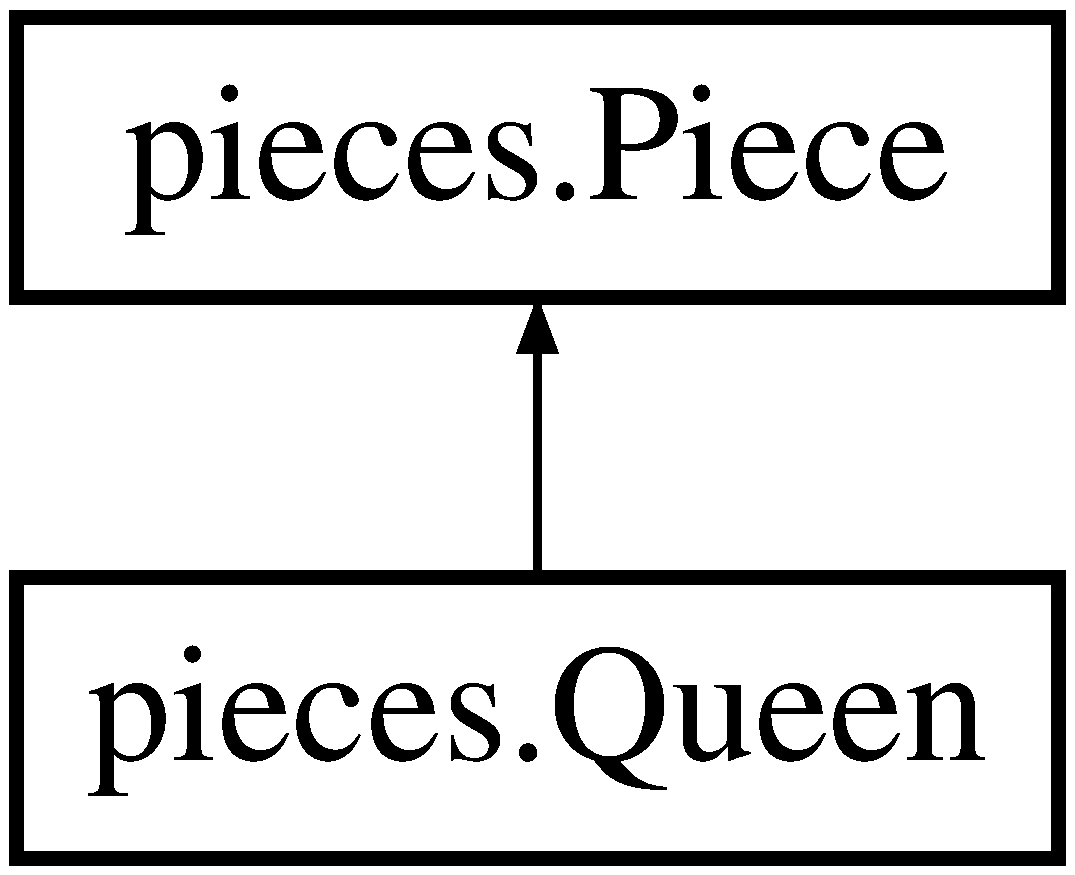
\includegraphics[height=2.000000cm]{classpieces_1_1_queen}
\end{center}
\end{figure}
\subsection*{Public Member Functions}
\begin{DoxyCompactItemize}
\item 
\hyperlink{classpieces_1_1_queen_a6165d27ad45f5a4b3819ace9c3fcecae}{Queen} (int \hyperlink{classpieces_1_1_piece_ae40d6201d0aed36f369dd9d8f55892e3}{piece\-Type}, Board my\-Board, int x, int y)
\item 
\hyperlink{classpieces_1_1_queen_a62084d8fc37c5ba7a23f6c174ab4b800}{Queen} (int \hyperlink{classpieces_1_1_piece_ae40d6201d0aed36f369dd9d8f55892e3}{piece\-Type})
\item 
boolean \hyperlink{classpieces_1_1_queen_a665a853e2c80719c12cbaf0c481c908a}{can\-Move\-Between} (Position start, Position end)
\end{DoxyCompactItemize}
\subsection*{Additional Inherited Members}


\subsection{Constructor \& Destructor Documentation}
\hypertarget{classpieces_1_1_queen_a6165d27ad45f5a4b3819ace9c3fcecae}{\index{pieces\-::\-Queen@{pieces\-::\-Queen}!Queen@{Queen}}
\index{Queen@{Queen}!pieces::Queen@{pieces\-::\-Queen}}
\subsubsection[{Queen}]{\setlength{\rightskip}{0pt plus 5cm}pieces.\-Queen.\-Queen (
\begin{DoxyParamCaption}
\item[{int}]{piece\-Type, }
\item[{Board}]{my\-Board, }
\item[{int}]{x, }
\item[{int}]{y}
\end{DoxyParamCaption}
)}}\label{classpieces_1_1_queen_a6165d27ad45f5a4b3819ace9c3fcecae}
Constructor No check to verify if piece\-Type is a \hyperlink{classpieces_1_1_queen}{Queen}. It is up to the caller to verify. \hypertarget{classpieces_1_1_queen_a62084d8fc37c5ba7a23f6c174ab4b800}{\index{pieces\-::\-Queen@{pieces\-::\-Queen}!Queen@{Queen}}
\index{Queen@{Queen}!pieces::Queen@{pieces\-::\-Queen}}
\subsubsection[{Queen}]{\setlength{\rightskip}{0pt plus 5cm}pieces.\-Queen.\-Queen (
\begin{DoxyParamCaption}
\item[{int}]{piece\-Type}
\end{DoxyParamCaption}
)}}\label{classpieces_1_1_queen_a62084d8fc37c5ba7a23f6c174ab4b800}
Constructor 

\subsection{Member Function Documentation}
\hypertarget{classpieces_1_1_queen_a665a853e2c80719c12cbaf0c481c908a}{\index{pieces\-::\-Queen@{pieces\-::\-Queen}!can\-Move\-Between@{can\-Move\-Between}}
\index{can\-Move\-Between@{can\-Move\-Between}!pieces::Queen@{pieces\-::\-Queen}}
\subsubsection[{can\-Move\-Between}]{\setlength{\rightskip}{0pt plus 5cm}boolean pieces.\-Queen.\-can\-Move\-Between (
\begin{DoxyParamCaption}
\item[{Position}]{start, }
\item[{Position}]{end}
\end{DoxyParamCaption}
)}}\label{classpieces_1_1_queen_a665a853e2c80719c12cbaf0c481c908a}
Check if the piece can move from start to end location. \begin{DoxyReturn}{Returns}
true if it can. false otherwise. 
\end{DoxyReturn}


The documentation for this class was generated from the following file\-:\begin{DoxyCompactItemize}
\item 
/\-Volumes/\-Shared/\-Dropbox/\-Fall 13/\-C\-S 242/workspace/\-Chess/pieces/\hyperlink{_queen_8java}{Queen.\-java}\end{DoxyCompactItemize}

\hypertarget{classpieces_1_1_rook}{\section{pieces.\-Rook Class Reference}
\label{classpieces_1_1_rook}\index{pieces.\-Rook@{pieces.\-Rook}}
}
Inheritance diagram for pieces.\-Rook\-:\begin{figure}[H]
\begin{center}
\leavevmode
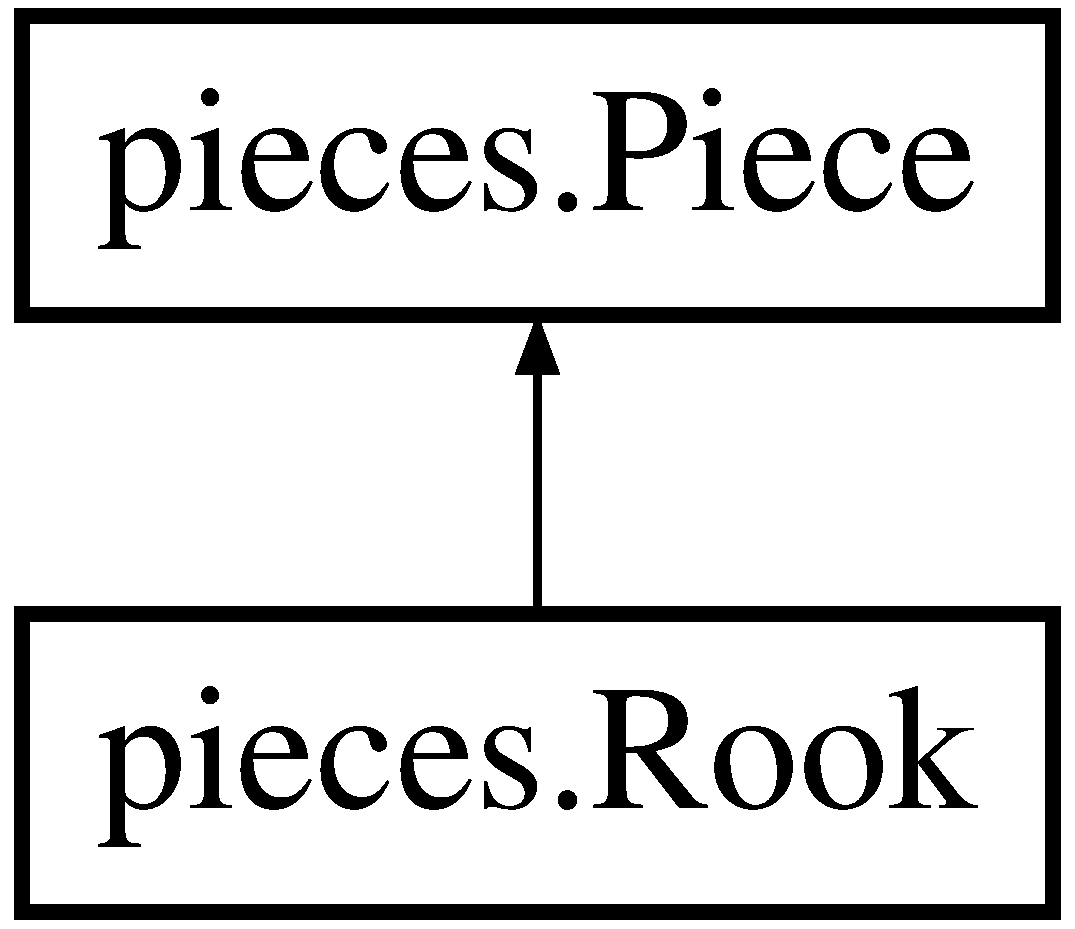
\includegraphics[height=2.000000cm]{classpieces_1_1_rook}
\end{center}
\end{figure}
\subsection*{Public Member Functions}
\begin{DoxyCompactItemize}
\item 
\hyperlink{classpieces_1_1_rook_a09c7380bb0b1e18f5e2b63a494c559f0}{Rook} (int \hyperlink{classpieces_1_1_piece_ae40d6201d0aed36f369dd9d8f55892e3}{piece\-Type}, Board my\-Board, int x, int y)
\item 
\hyperlink{classpieces_1_1_rook_ad49559ea874f947761af67e428098500}{Rook} (int \hyperlink{classpieces_1_1_piece_ae40d6201d0aed36f369dd9d8f55892e3}{piece\-Type})
\item 
boolean \hyperlink{classpieces_1_1_rook_a79a453f36c4582ccadbdc1ea5e01d5ad}{can\-Move\-Between} (Position start, Position end)
\end{DoxyCompactItemize}
\subsection*{Additional Inherited Members}


\subsection{Constructor \& Destructor Documentation}
\hypertarget{classpieces_1_1_rook_a09c7380bb0b1e18f5e2b63a494c559f0}{\index{pieces\-::\-Rook@{pieces\-::\-Rook}!Rook@{Rook}}
\index{Rook@{Rook}!pieces::Rook@{pieces\-::\-Rook}}
\subsubsection[{Rook}]{\setlength{\rightskip}{0pt plus 5cm}pieces.\-Rook.\-Rook (
\begin{DoxyParamCaption}
\item[{int}]{piece\-Type, }
\item[{Board}]{my\-Board, }
\item[{int}]{x, }
\item[{int}]{y}
\end{DoxyParamCaption}
)}}\label{classpieces_1_1_rook_a09c7380bb0b1e18f5e2b63a494c559f0}
Constructor No check to verify if piece\-Type is a \hyperlink{classpieces_1_1_rook}{Rook}. It is up to the caller to verify. \hypertarget{classpieces_1_1_rook_ad49559ea874f947761af67e428098500}{\index{pieces\-::\-Rook@{pieces\-::\-Rook}!Rook@{Rook}}
\index{Rook@{Rook}!pieces::Rook@{pieces\-::\-Rook}}
\subsubsection[{Rook}]{\setlength{\rightskip}{0pt plus 5cm}pieces.\-Rook.\-Rook (
\begin{DoxyParamCaption}
\item[{int}]{piece\-Type}
\end{DoxyParamCaption}
)}}\label{classpieces_1_1_rook_ad49559ea874f947761af67e428098500}
Constructor 

\subsection{Member Function Documentation}
\hypertarget{classpieces_1_1_rook_a79a453f36c4582ccadbdc1ea5e01d5ad}{\index{pieces\-::\-Rook@{pieces\-::\-Rook}!can\-Move\-Between@{can\-Move\-Between}}
\index{can\-Move\-Between@{can\-Move\-Between}!pieces::Rook@{pieces\-::\-Rook}}
\subsubsection[{can\-Move\-Between}]{\setlength{\rightskip}{0pt plus 5cm}boolean pieces.\-Rook.\-can\-Move\-Between (
\begin{DoxyParamCaption}
\item[{Position}]{start, }
\item[{Position}]{end}
\end{DoxyParamCaption}
)}}\label{classpieces_1_1_rook_a79a453f36c4582ccadbdc1ea5e01d5ad}
Check if the piece can move from start to end location. \begin{DoxyReturn}{Returns}
true if it can. false otherwise. 
\end{DoxyReturn}


The documentation for this class was generated from the following file\-:\begin{DoxyCompactItemize}
\item 
/\-Volumes/\-Shared/\-Dropbox/\-Fall 13/\-C\-S 242/workspace/\-Chess/pieces/\hyperlink{_rook_8java}{Rook.\-java}\end{DoxyCompactItemize}

\hypertarget{classgame_1_1_game_1_1_state}{\section{game.\-Game.\-State Class Reference}
\label{classgame_1_1_game_1_1_state}\index{game.\-Game.\-State@{game.\-Game.\-State}}
}
\subsection*{Public Member Functions}
\begin{DoxyCompactItemize}
\item 
\hyperlink{classgame_1_1_game_1_1_state_acd7e7c52d8be9391c072ad7f17d8bfbd}{State} ()
\item 
\hyperlink{classgame_1_1_game_1_1_state_a543a3e52fe95dbb4615d402046516814}{State} (\hyperlink{classgame_1_1_game_1_1_state}{State} s)
\item 
void \hyperlink{classgame_1_1_game_1_1_state_acff6fcbfc126e2cddddf2039c23d50f7}{set\-State} (Move last\-Move, \hyperlink{classpieces_1_1_piece}{Piece} piece\-Moved, \hyperlink{classpieces_1_1_piece}{Piece} last\-Captured)
\item 
boolean \hyperlink{classgame_1_1_game_1_1_state_abfc8d34239b12d839f80abe4eb68a23c}{is\-In\-Check} ()
\item 
int \hyperlink{classgame_1_1_game_1_1_state_a1a4697dba2d94faee2cfacf138d3b9c1}{get\-Checked\-Color} ()
\item 
int \hyperlink{classgame_1_1_game_1_1_state_a1bc13e0e8116b07f9bba89881ac78084}{get\-Turn} ()
\end{DoxyCompactItemize}
\subsection*{Private Attributes}
\begin{DoxyCompactItemize}
\item 
int \hyperlink{classgame_1_1_game_1_1_state_a3cc50de4b7853ee4dfcd559a29ffffd3}{turn} = 1
\end{DoxyCompactItemize}


\subsection{Detailed Description}
\hyperlink{classgame_1_1_game_1_1_state}{State} stores information at a specific point in the game. \begin{DoxyAuthor}{Author}
Shashank Bharadwaj 
\end{DoxyAuthor}


\subsection{Constructor \& Destructor Documentation}
\hypertarget{classgame_1_1_game_1_1_state_acd7e7c52d8be9391c072ad7f17d8bfbd}{\index{game\-::\-Game\-::\-State@{game\-::\-Game\-::\-State}!State@{State}}
\index{State@{State}!game::Game::State@{game\-::\-Game\-::\-State}}
\subsubsection[{State}]{\setlength{\rightskip}{0pt plus 5cm}game.\-Game.\-State.\-State (
\begin{DoxyParamCaption}
{}
\end{DoxyParamCaption}
)}}\label{classgame_1_1_game_1_1_state_acd7e7c52d8be9391c072ad7f17d8bfbd}
Empty constructor \hypertarget{classgame_1_1_game_1_1_state_a543a3e52fe95dbb4615d402046516814}{\index{game\-::\-Game\-::\-State@{game\-::\-Game\-::\-State}!State@{State}}
\index{State@{State}!game::Game::State@{game\-::\-Game\-::\-State}}
\subsubsection[{State}]{\setlength{\rightskip}{0pt plus 5cm}game.\-Game.\-State.\-State (
\begin{DoxyParamCaption}
\item[{{\bf State}}]{s}
\end{DoxyParamCaption}
)}}\label{classgame_1_1_game_1_1_state_a543a3e52fe95dbb4615d402046516814}
Constructor 

\subsection{Member Function Documentation}
\hypertarget{classgame_1_1_game_1_1_state_a1a4697dba2d94faee2cfacf138d3b9c1}{\index{game\-::\-Game\-::\-State@{game\-::\-Game\-::\-State}!get\-Checked\-Color@{get\-Checked\-Color}}
\index{get\-Checked\-Color@{get\-Checked\-Color}!game::Game::State@{game\-::\-Game\-::\-State}}
\subsubsection[{get\-Checked\-Color}]{\setlength{\rightskip}{0pt plus 5cm}int game.\-Game.\-State.\-get\-Checked\-Color (
\begin{DoxyParamCaption}
{}
\end{DoxyParamCaption}
)}}\label{classgame_1_1_game_1_1_state_a1a4697dba2d94faee2cfacf138d3b9c1}
\hypertarget{classgame_1_1_game_1_1_state_a1bc13e0e8116b07f9bba89881ac78084}{\index{game\-::\-Game\-::\-State@{game\-::\-Game\-::\-State}!get\-Turn@{get\-Turn}}
\index{get\-Turn@{get\-Turn}!game::Game::State@{game\-::\-Game\-::\-State}}
\subsubsection[{get\-Turn}]{\setlength{\rightskip}{0pt plus 5cm}int game.\-Game.\-State.\-get\-Turn (
\begin{DoxyParamCaption}
{}
\end{DoxyParamCaption}
)}}\label{classgame_1_1_game_1_1_state_a1bc13e0e8116b07f9bba89881ac78084}
\hypertarget{classgame_1_1_game_1_1_state_abfc8d34239b12d839f80abe4eb68a23c}{\index{game\-::\-Game\-::\-State@{game\-::\-Game\-::\-State}!is\-In\-Check@{is\-In\-Check}}
\index{is\-In\-Check@{is\-In\-Check}!game::Game::State@{game\-::\-Game\-::\-State}}
\subsubsection[{is\-In\-Check}]{\setlength{\rightskip}{0pt plus 5cm}boolean game.\-Game.\-State.\-is\-In\-Check (
\begin{DoxyParamCaption}
{}
\end{DoxyParamCaption}
)}}\label{classgame_1_1_game_1_1_state_abfc8d34239b12d839f80abe4eb68a23c}
\hypertarget{classgame_1_1_game_1_1_state_acff6fcbfc126e2cddddf2039c23d50f7}{\index{game\-::\-Game\-::\-State@{game\-::\-Game\-::\-State}!set\-State@{set\-State}}
\index{set\-State@{set\-State}!game::Game::State@{game\-::\-Game\-::\-State}}
\subsubsection[{set\-State}]{\setlength{\rightskip}{0pt plus 5cm}void game.\-Game.\-State.\-set\-State (
\begin{DoxyParamCaption}
\item[{Move}]{last\-Move, }
\item[{{\bf Piece}}]{piece\-Moved, }
\item[{{\bf Piece}}]{last\-Captured}
\end{DoxyParamCaption}
)}}\label{classgame_1_1_game_1_1_state_acff6fcbfc126e2cddddf2039c23d50f7}


\subsection{Member Data Documentation}
\hypertarget{classgame_1_1_game_1_1_state_a3cc50de4b7853ee4dfcd559a29ffffd3}{\index{game\-::\-Game\-::\-State@{game\-::\-Game\-::\-State}!turn@{turn}}
\index{turn@{turn}!game::Game::State@{game\-::\-Game\-::\-State}}
\subsubsection[{turn}]{\setlength{\rightskip}{0pt plus 5cm}int game.\-Game.\-State.\-turn = 1\hspace{0.3cm}{\ttfamily [private]}}}\label{classgame_1_1_game_1_1_state_a3cc50de4b7853ee4dfcd559a29ffffd3}


The documentation for this class was generated from the following file\-:\begin{DoxyCompactItemize}
\item 
/\-Volumes/\-Shared/\-Dropbox/\-Fall 13/\-C\-S 242/workspace/\-Chess/game/\hyperlink{_game_8java}{Game.\-java}\end{DoxyCompactItemize}

\chapter{File Documentation}
\hypertarget{_board_8java}{\section{/\-Volumes/\-Shared/\-Dropbox/\-Fall 13/\-C\-S 242/workspace/\-Chess/game/\-Board.java File Reference}
\label{_board_8java}\index{/\-Volumes/\-Shared/\-Dropbox/\-Fall 13/\-C\-S 242/workspace/\-Chess/game/\-Board.\-java@{/\-Volumes/\-Shared/\-Dropbox/\-Fall 13/\-C\-S 242/workspace/\-Chess/game/\-Board.\-java}}
}
\subsection*{Classes}
\begin{DoxyCompactItemize}
\item 
class \hyperlink{classgame_1_1_board}{game.\-Board}
\end{DoxyCompactItemize}
\subsection*{Packages}
\begin{DoxyCompactItemize}
\item 
package \hyperlink{namespacegame}{game}
\end{DoxyCompactItemize}

\hypertarget{_game_8java}{\section{/\-Volumes/\-Shared/\-Dropbox/\-Fall 13/\-C\-S 242/workspace/\-Chess/game/\-Game.java File Reference}
\label{_game_8java}\index{/\-Volumes/\-Shared/\-Dropbox/\-Fall 13/\-C\-S 242/workspace/\-Chess/game/\-Game.\-java@{/\-Volumes/\-Shared/\-Dropbox/\-Fall 13/\-C\-S 242/workspace/\-Chess/game/\-Game.\-java}}
}
\subsection*{Classes}
\begin{DoxyCompactItemize}
\item 
class \hyperlink{classgame_1_1_game}{game.\-Game}
\item 
class \hyperlink{classgame_1_1_game_1_1_state}{game.\-Game.\-State}
\end{DoxyCompactItemize}
\subsection*{Packages}
\begin{DoxyCompactItemize}
\item 
package \hyperlink{namespacegame}{game}
\end{DoxyCompactItemize}

\hypertarget{_player_8java}{\section{/\-Volumes/\-Shared/\-Dropbox/\-Fall 13/\-C\-S 242/workspace/\-Chess/game/\-Player.java File Reference}
\label{_player_8java}\index{/\-Volumes/\-Shared/\-Dropbox/\-Fall 13/\-C\-S 242/workspace/\-Chess/game/\-Player.\-java@{/\-Volumes/\-Shared/\-Dropbox/\-Fall 13/\-C\-S 242/workspace/\-Chess/game/\-Player.\-java}}
}
\subsection*{Classes}
\begin{DoxyCompactItemize}
\item 
class \hyperlink{classgame_1_1_player}{game.\-Player}
\end{DoxyCompactItemize}
\subsection*{Packages}
\begin{DoxyCompactItemize}
\item 
package \hyperlink{namespacegame}{game}
\end{DoxyCompactItemize}

\hypertarget{_position_8java}{\section{/\-Volumes/\-Shared/\-Dropbox/\-Fall 13/\-C\-S 242/workspace/\-Chess/game/\-Position.java File Reference}
\label{_position_8java}\index{/\-Volumes/\-Shared/\-Dropbox/\-Fall 13/\-C\-S 242/workspace/\-Chess/game/\-Position.\-java@{/\-Volumes/\-Shared/\-Dropbox/\-Fall 13/\-C\-S 242/workspace/\-Chess/game/\-Position.\-java}}
}
\subsection*{Classes}
\begin{DoxyCompactItemize}
\item 
class \hyperlink{classgame_1_1_position}{game.\-Position}
\item 
class {\bfseries game.\-Move}
\end{DoxyCompactItemize}
\subsection*{Packages}
\begin{DoxyCompactItemize}
\item 
package \hyperlink{namespacegame}{game}
\end{DoxyCompactItemize}

\hypertarget{_bishop_8java}{\section{/\-Volumes/\-Shared/\-Dropbox/\-Fall 13/\-C\-S 242/workspace/\-Chess/pieces/\-Bishop.java File Reference}
\label{_bishop_8java}\index{/\-Volumes/\-Shared/\-Dropbox/\-Fall 13/\-C\-S 242/workspace/\-Chess/pieces/\-Bishop.\-java@{/\-Volumes/\-Shared/\-Dropbox/\-Fall 13/\-C\-S 242/workspace/\-Chess/pieces/\-Bishop.\-java}}
}
\subsection*{Classes}
\begin{DoxyCompactItemize}
\item 
class \hyperlink{classpieces_1_1_bishop}{pieces.\-Bishop}
\end{DoxyCompactItemize}
\subsection*{Packages}
\begin{DoxyCompactItemize}
\item 
package \hyperlink{namespacepieces}{pieces}
\end{DoxyCompactItemize}

\hypertarget{_fly_8java}{\section{/\-Volumes/\-Shared/\-Dropbox/\-Fall 13/\-C\-S 242/workspace/\-Chess/pieces/\-Fly.java File Reference}
\label{_fly_8java}\index{/\-Volumes/\-Shared/\-Dropbox/\-Fall 13/\-C\-S 242/workspace/\-Chess/pieces/\-Fly.\-java@{/\-Volumes/\-Shared/\-Dropbox/\-Fall 13/\-C\-S 242/workspace/\-Chess/pieces/\-Fly.\-java}}
}
\subsection*{Classes}
\begin{DoxyCompactItemize}
\item 
class \hyperlink{classpieces_1_1_fly}{pieces.\-Fly}
\end{DoxyCompactItemize}
\subsection*{Packages}
\begin{DoxyCompactItemize}
\item 
package \hyperlink{namespacepieces}{pieces}
\end{DoxyCompactItemize}

\hypertarget{_fly_trap_8java}{\section{/\-Volumes/\-Shared/\-Dropbox/\-Fall 13/\-C\-S 242/workspace/\-Chess/pieces/\-Fly\-Trap.java File Reference}
\label{_fly_trap_8java}\index{/\-Volumes/\-Shared/\-Dropbox/\-Fall 13/\-C\-S 242/workspace/\-Chess/pieces/\-Fly\-Trap.\-java@{/\-Volumes/\-Shared/\-Dropbox/\-Fall 13/\-C\-S 242/workspace/\-Chess/pieces/\-Fly\-Trap.\-java}}
}
\subsection*{Classes}
\begin{DoxyCompactItemize}
\item 
class \hyperlink{classpieces_1_1_fly_trap}{pieces.\-Fly\-Trap}
\end{DoxyCompactItemize}
\subsection*{Packages}
\begin{DoxyCompactItemize}
\item 
package \hyperlink{namespacepieces}{pieces}
\end{DoxyCompactItemize}

\hypertarget{_king_8java}{\section{/\-Volumes/\-Shared/\-Dropbox/\-Fall 13/\-C\-S 242/workspace/\-Chess/pieces/\-King.java File Reference}
\label{_king_8java}\index{/\-Volumes/\-Shared/\-Dropbox/\-Fall 13/\-C\-S 242/workspace/\-Chess/pieces/\-King.\-java@{/\-Volumes/\-Shared/\-Dropbox/\-Fall 13/\-C\-S 242/workspace/\-Chess/pieces/\-King.\-java}}
}
\subsection*{Classes}
\begin{DoxyCompactItemize}
\item 
class \hyperlink{classpieces_1_1_king}{pieces.\-King}
\end{DoxyCompactItemize}
\subsection*{Packages}
\begin{DoxyCompactItemize}
\item 
package \hyperlink{namespacepieces}{pieces}
\end{DoxyCompactItemize}

\hypertarget{_knight_8java}{\section{/\-Volumes/\-Shared/\-Dropbox/\-Fall 13/\-C\-S 242/workspace/\-Chess/pieces/\-Knight.java File Reference}
\label{_knight_8java}\index{/\-Volumes/\-Shared/\-Dropbox/\-Fall 13/\-C\-S 242/workspace/\-Chess/pieces/\-Knight.\-java@{/\-Volumes/\-Shared/\-Dropbox/\-Fall 13/\-C\-S 242/workspace/\-Chess/pieces/\-Knight.\-java}}
}
\subsection*{Classes}
\begin{DoxyCompactItemize}
\item 
class \hyperlink{classpieces_1_1_knight}{pieces.\-Knight}
\end{DoxyCompactItemize}
\subsection*{Packages}
\begin{DoxyCompactItemize}
\item 
package \hyperlink{namespacepieces}{pieces}
\end{DoxyCompactItemize}

\hypertarget{_pawn_8java}{\section{/\-Volumes/\-Shared/\-Dropbox/\-Fall 13/\-C\-S 242/workspace/\-Chess/pieces/\-Pawn.java File Reference}
\label{_pawn_8java}\index{/\-Volumes/\-Shared/\-Dropbox/\-Fall 13/\-C\-S 242/workspace/\-Chess/pieces/\-Pawn.\-java@{/\-Volumes/\-Shared/\-Dropbox/\-Fall 13/\-C\-S 242/workspace/\-Chess/pieces/\-Pawn.\-java}}
}
\subsection*{Classes}
\begin{DoxyCompactItemize}
\item 
class \hyperlink{classpieces_1_1_pawn}{pieces.\-Pawn}
\end{DoxyCompactItemize}
\subsection*{Packages}
\begin{DoxyCompactItemize}
\item 
package \hyperlink{namespacepieces}{pieces}
\end{DoxyCompactItemize}

\hypertarget{_piece_8java}{\section{/\-Volumes/\-Shared/\-Dropbox/\-Fall 13/\-C\-S 242/workspace/\-Chess/pieces/\-Piece.java File Reference}
\label{_piece_8java}\index{/\-Volumes/\-Shared/\-Dropbox/\-Fall 13/\-C\-S 242/workspace/\-Chess/pieces/\-Piece.\-java@{/\-Volumes/\-Shared/\-Dropbox/\-Fall 13/\-C\-S 242/workspace/\-Chess/pieces/\-Piece.\-java}}
}
\subsection*{Classes}
\begin{DoxyCompactItemize}
\item 
class \hyperlink{classpieces_1_1_piece}{pieces.\-Piece}
\end{DoxyCompactItemize}
\subsection*{Packages}
\begin{DoxyCompactItemize}
\item 
package \hyperlink{namespacepieces}{pieces}
\end{DoxyCompactItemize}

\hypertarget{_queen_8java}{\section{/\-Volumes/\-Shared/\-Dropbox/\-Fall 13/\-C\-S 242/workspace/\-Chess/pieces/\-Queen.java File Reference}
\label{_queen_8java}\index{/\-Volumes/\-Shared/\-Dropbox/\-Fall 13/\-C\-S 242/workspace/\-Chess/pieces/\-Queen.\-java@{/\-Volumes/\-Shared/\-Dropbox/\-Fall 13/\-C\-S 242/workspace/\-Chess/pieces/\-Queen.\-java}}
}
\subsection*{Classes}
\begin{DoxyCompactItemize}
\item 
class \hyperlink{classpieces_1_1_queen}{pieces.\-Queen}
\end{DoxyCompactItemize}
\subsection*{Packages}
\begin{DoxyCompactItemize}
\item 
package \hyperlink{namespacepieces}{pieces}
\end{DoxyCompactItemize}

\hypertarget{_rook_8java}{\section{/\-Volumes/\-Shared/\-Dropbox/\-Fall 13/\-C\-S 242/workspace/\-Chess/pieces/\-Rook.java File Reference}
\label{_rook_8java}\index{/\-Volumes/\-Shared/\-Dropbox/\-Fall 13/\-C\-S 242/workspace/\-Chess/pieces/\-Rook.\-java@{/\-Volumes/\-Shared/\-Dropbox/\-Fall 13/\-C\-S 242/workspace/\-Chess/pieces/\-Rook.\-java}}
}
\subsection*{Classes}
\begin{DoxyCompactItemize}
\item 
class \hyperlink{classpieces_1_1_rook}{pieces.\-Rook}
\end{DoxyCompactItemize}
\subsection*{Packages}
\begin{DoxyCompactItemize}
\item 
package \hyperlink{namespacepieces}{pieces}
\end{DoxyCompactItemize}

%--- End generated contents ---

% Index
\newpage
\phantomsection
\addcontentsline{toc}{part}{Index}
\printindex

\end{document}
